% =====================================================================
% Project B3 -- central slide deck for the 60-minute talk (Wed 2 Dec 2026)
% Overleaf: compiler pdfLaTeX, main document main.tex.
%
% Who edits what (one file per section, so nobody overwrites anybody):
%   sections/00-opening.tex          T3  title, draft status, roadmap
%   sections/01-motivation.tex       T3  6 min
%   sections/02-kd-basics.tex        T2  8 min
%   sections/03-kl-onpolicy.tex      T1  6 min
%   sections/04-literature.tex       E2  8 min
%   sections/05-design.tex           T3 4, T2 2, T1 4 min (incl. pipeline)
%   sections/06-evaluation.tex       E2 2, E1 2 min
%   sections/07-results.tex          E1 6, E3 4 min
%   sections/08-interpretation.tex   E1 2, E3 3 min
%   sections/09-conclusion.tex       E3 3 min (+ T3 traceability slide)
%   sections/10-backup.tex           backup slides and references
%
% Shared colours and macros: preamble.tex (owner T3).
% Orange "To add" boxes mark content that is missing from the repository
% or still has to be written. Replace each box when the content exists.
% =====================================================================
\documentclass[aspectratio=169,10pt]{beamer}
% =====================================================================
% preamble.tex -- shared look and helper commands for the B3 slide deck
% Owner: T3 (slides lead). Change this file only after telling the team:
% every section file depends on the colours and macros below.
% Compile with pdfLaTeX (Overleaf default).
% =====================================================================

\usepackage[T1]{fontenc}
\usepackage{lmodern}
\usepackage{amsmath,amssymb}
\usepackage{booktabs}
\usepackage{array}
\usepackage{tikz}
\usetikzlibrary{arrows.meta,positioning,calc,shapes.geometric,fit,backgrounds}
\usepackage{pgfplots}
\pgfplotsset{compat=1.18}
\usepackage{listings}
\usepackage[most]{tcolorbox}
\usepackage{appendixnumberbeamer}

% ---------------------------------------------------------------------
% Colour palette (light theme)
% ---------------------------------------------------------------------
\definecolor{kdnavy}{HTML}{1F3A5F}    % headings
\definecolor{kdblue}{HTML}{2F6DB5}    % structure, main data series
\definecolor{kdpale}{HTML}{EAF1FB}    % title band, block titles
\definecolor{kdpaler}{HTML}{F5F8FD}   % block bodies
\definecolor{kdteal}{HTML}{178F87}    % second data series, "Ours"
\definecolor{kdorange}{HTML}{D9731A}  % accent, baselines, to-do boxes
\definecolor{kdred}{HTML}{C0392B}     % errors, warnings
\definecolor{kdgray}{HTML}{5B6575}    % muted text
\definecolor{kdlight}{HTML}{F2F4F7}   % footline
\definecolor{kdink}{HTML}{1E2430}     % body text
\definecolor{kdcode}{HTML}{F6F8FA}    % code background
\definecolor{kdtodo}{HTML}{FFF6E8}    % to-do box background

% ---------------------------------------------------------------------
% Beamer colours, fonts and templates
% ---------------------------------------------------------------------
\setbeamertemplate{navigation symbols}{}
\setbeamercolor{normal text}{fg=kdink,bg=white}
\setbeamercolor{structure}{fg=kdblue}
\setbeamercolor{alerted text}{fg=kdorange}
\setbeamercolor{frametitle}{fg=kdnavy,bg=kdpale}
\setbeamercolor{framesubtitle}{fg=kdgray}
\setbeamercolor{title}{fg=kdnavy}
\setbeamercolor{subtitle}{fg=kdblue}
\setbeamercolor{block title}{fg=kdnavy,bg=kdpale}
\setbeamercolor{block body}{fg=kdink,bg=kdpaler}
\setbeamercolor{block title alerted}{fg=white,bg=kdorange}
\setbeamercolor{block body alerted}{fg=kdink,bg=kdtodo}
\setbeamercolor{block title example}{fg=white,bg=kdteal}
\setbeamercolor{block body example}{fg=kdink,bg=kdteal!6}
\setbeamercolor{footline}{fg=kdgray,bg=kdlight}
\setbeamercolor{item}{fg=kdblue}
\setbeamercolor{section in toc}{fg=kdnavy}
\setbeamercolor{section in toc shaded}{fg=kdgray}

\setbeamerfont{frametitle}{size=\large,series=\bfseries}
\setbeamerfont{framesubtitle}{size=\footnotesize,series=\mdseries}
\setbeamerfont{footline}{size=\tiny}
\setbeamerfont{block title}{size=\small,series=\bfseries}

\setbeamertemplate{itemize items}[circle]
\setbeamertemplate{enumerate items}[default]
\setbeamertemplate{blocks}[rounded]
\setbeamertemplate{section in toc}[sections numbered]
\setbeamertemplate{section in toc shaded}[default][40]

% Frame title: a pale band across the slide with a thin blue rule below.
\makeatletter
\setbeamertemplate{frametitle}{%
  \nointerlineskip
  \begin{beamercolorbox}[wd=\paperwidth,leftskip=0.5cm,rightskip=0.5cm,sep=0.2cm]{frametitle}%
    \usebeamerfont{frametitle}\strut\insertframetitle\strut
    \ifx\insertframesubtitle\@empty\else
      \par{\usebeamerfont{framesubtitle}\usebeamercolor[fg]{framesubtitle}\insertframesubtitle\strut\par}%
    \fi
  \end{beamercolorbox}%
  \nointerlineskip
  \hbox{\color{kdblue}\rule{\paperwidth}{0.6pt}}%
  \vskip0.1cm
}
\makeatother

% Footline: project name, current section, slide number.
\setbeamertemplate{footline}{%
  \leavevmode%
  \hbox{%
    \begin{beamercolorbox}[wd=.40\paperwidth,ht=2.4ex,dp=1ex,leftskip=0.5cm]{footline}%
      \usebeamerfont{footline}Project B3 $\cdot$ Knowledge Distillation
    \end{beamercolorbox}%
    \begin{beamercolorbox}[wd=.40\paperwidth,ht=2.4ex,dp=1ex,center]{footline}%
      \usebeamerfont{footline}\insertsectionhead
    \end{beamercolorbox}%
    \begin{beamercolorbox}[wd=.20\paperwidth,ht=2.4ex,dp=1ex,right,rightskip=0.5cm]{footline}%
      \usebeamerfont{footline}\insertframenumber{} / \inserttotalframenumber
    \end{beamercolorbox}}%
  \vskip0pt%
}

% Section divider: big number, section title, presenter and minutes,
% and the roadmap with the current section highlighted.
% Each section file sets \sectioninfo just before its \section command.
\newcommand{\sectioninfo}{}
\AtBeginSection[]{%
  \begin{frame}[plain,noframenumbering]
    \begin{tikzpicture}[remember picture,overlay]
      \fill[kdpaler] (current page.north west) rectangle (current page.south east);
      \fill[kdblue] (current page.north west) rectangle ([xshift=0.22cm]current page.south west);
    \end{tikzpicture}%
    \begin{columns}[c]
      \begin{column}{0.52\textwidth}
        {\color{kdblue}\fontsize{38}{40}\selectfont\bfseries\thesection\par}
        \vspace{0.2cm}
        {\color{kdnavy}\Large\bfseries\insertsectionhead\par}
        \vspace{0.3cm}
        {\color{kdgray}\normalsize\sectioninfo\par}
      \end{column}
      \begin{column}{0.42\textwidth}
        \scriptsize\tableofcontents[currentsection,hideallsubsections]
      \end{column}
    \end{columns}
  \end{frame}
}

% ---------------------------------------------------------------------
% Helper commands used on the slides
% ---------------------------------------------------------------------
% Small coloured labels for frame titles:
%   \est  = claim taken from the literature
%   \ours = result from our own runs (a file in results/)
%   \who{T3} = who presents this slide
\newcommand{\badge}[2]{{\setlength{\fboxsep}{1.6pt}\colorbox{#1}{\textcolor{white}{\scriptsize\bfseries\strut #2}}}}
\newcommand{\est}{\badge{kdblue}{Established}}
\newcommand{\ours}{\badge{kdteal}{Ours}}
\newcommand{\who}[1]{\badge{kdgray}{#1}}
% A source in grey after a statement: \src{Hinton et al., 2015}
\newcommand{\src}[1]{{\color{kdgray}\scriptsize(#1)}}
% Arm names in typewriter type
\newcommand{\arm}[1]{\texttt{#1}}
% A path or file in the repository (not \path: TikZ already uses that name)
\newcommand{\repofile}[1]{{\color{kdnavy}\texttt{#1}}}

% To-do box: marks content that is missing from the repository or still
% has to be written. Replace the box with real content when it exists.
%   \begin{todobox}{Seed 1 results (T1)} what is needed ... \end{todobox}
\newtcolorbox{todobox}[1]{enhanced,colback=kdtodo,colframe=kdorange,
  boxrule=0.6pt,arc=2pt,left=5pt,right=5pt,top=3pt,bottom=3pt,
  coltitle=white,colbacktitle=kdorange,fonttitle=\bfseries\scriptsize,
  title={To add: #1},fontupper=\scriptsize}

% Info box for short key messages
\newtcolorbox{keybox}{enhanced,colback=kdpale,colframe=kdblue,
  boxrule=0.6pt,arc=2pt,left=6pt,right=6pt,top=4pt,bottom=4pt,fontupper=\small}

% ---------------------------------------------------------------------
% TikZ helpers
% ---------------------------------------------------------------------
% "visible on=<2->" shows a TikZ element from overlay 2 onwards while
% keeping its space reserved, so the picture does not jump.
\tikzset{
  invisible/.style={opacity=0,text opacity=0},
  visible on/.style={alt={#1{}{invisible}}},
  alt/.code args={<#1>#2#3}{\alt<#1>{\pgfkeysalso{#2}}{\pgfkeysalso{#3}}},
  stage/.style={draw=kdblue,fill=kdpale,rounded corners=3pt,align=center,
    font=\scriptsize,text width=1.85cm,minimum height=1.15cm,inner sep=3pt},
  stageT/.style={stage,draw=kdteal,fill=kdteal!8},
  stageX/.style={stage,draw=kdorange,fill=kdtodo,dashed},
  flow/.style={-{Stealth[length=2mm]},thick,draw=kdgray},
  filelabel/.style={font=\tiny\ttfamily,text=kdgray,align=center},
}

% pgfplots defaults for this deck
\pgfplotsset{
  kdaxis/.style={
    axis line style={kdgray},
    tick style={kdgray},
    tick label style={font=\scriptsize,text=kdink},
    label style={font=\scriptsize,text=kdink},
    legend style={font=\scriptsize,draw=none,fill=none},
    title style={font=\small\bfseries,text=kdnavy},
    major grid style={kdlight},
  },
}

% ---------------------------------------------------------------------
% Code listings
% ---------------------------------------------------------------------
\lstdefinestyle{kdpy}{
  language=Python,
  basicstyle=\ttfamily\scriptsize,
  keywordstyle=\color{kdblue}\bfseries,
  commentstyle=\color{kdgray}\itshape,
  stringstyle=\color{kdteal},
  backgroundcolor=\color{kdcode},
  frame=single,framerule=0.4pt,rulecolor=\color{kdpale},
  xleftmargin=3pt,xrightmargin=3pt,
  showstringspaces=false,columns=fullflexible,keepspaces=true,
  breaklines=true,tabsize=4,aboveskip=3pt,belowskip=3pt,upquote=true,
}
\lstdefinestyle{kdplain}{
  style=kdpy,language={},
  morecomment=[l]{\#},
}
\lstset{style=kdpy}


\title{Whose Text Should a Small Model Practise On?}
\subtitle{Distilling Qwen3-4B into Qwen3-0.6B on GSM8K}
\author{Team B3: T1, T2, T3, E1, E2, E3 \quad{\color{kdorange}(add names)}}
\institute{AAI2 Practical Project B3: Knowledge Distillation and Model Compression}
\date{Wednesday 2 December 2026}

\begin{document}

% =====================================================================
% 00-opening.tex -- title, draft status, roadmap.  Owner: T3
% =====================================================================

% ---------------------------------------------------------------- title
\begin{frame}[plain,noframenumbering]
  \begin{tikzpicture}[remember picture,overlay]
    \fill[kdpale] (current page.south west) rectangle ([yshift=1.0cm]current page.south east);
    \fill[kdblue] (current page.north west) rectangle ([xshift=0.22cm]current page.south west);
    \node[anchor=south west,font=\scriptsize,text=kdnavy]
      at ([xshift=0.8cm,yshift=0.38cm]current page.south west) {\insertinstitute};
  \end{tikzpicture}%
  \begin{columns}[c]
    \begin{column}{0.53\textwidth}
      {\color{kdnavy}\LARGE\bfseries \inserttitle\par}
      \vspace{0.35cm}
      {\color{kdblue}\large \insertsubtitle\par}
      \vspace{0.6cm}
      {\small \insertauthor\par}
      \vspace{0.15cm}
      {\small\color{kdgray} \insertdate\par}
      \vspace{0.9cm}
    \end{column}
    \begin{column}{0.43\textwidth}
      \centering
      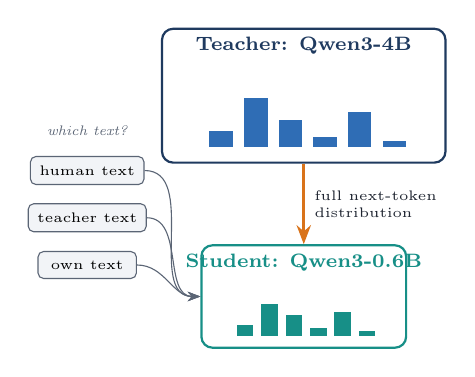
\begin{tikzpicture}[font=\scriptsize]
        % teacher with its next-token distribution
        \node[draw=kdnavy,line width=0.8pt,fill=white,rounded corners=4pt,
              minimum width=3.6cm,minimum height=1.7cm] (T) at (0,2.0) {};
        \node[anchor=north,font=\scriptsize\bfseries,text=kdnavy] at (T.north) {Teacher: Qwen3-4B};
        \foreach \i/\h in {0/0.20,1/0.62,2/0.34,3/0.12,4/0.44,5/0.07}
          \fill[kdblue] (-1.2+\i*0.44,1.35) rectangle ++(0.30,\h);
        % student, a smaller copy of the distribution
        \node[draw=kdteal,line width=0.8pt,fill=white,rounded corners=4pt,
              minimum width=2.6cm,minimum height=1.3cm] (S) at (0,-0.55) {};
        \node[anchor=north,font=\scriptsize\bfseries,text=kdteal] at (S.north) {Student: Qwen3-0.6B};
        \foreach \i/\h in {0/0.14,1/0.40,2/0.26,3/0.10,4/0.30,5/0.06}
          \fill[kdteal] (-0.85+\i*0.31,-1.05) rectangle ++(0.21,\h);
        % the distillation signal
        \draw[-{Stealth[length=2.4mm]},very thick,kdorange] (T.south) -- (S.north)
          node[midway,right,align=left,text=kdink,font=\tiny] {full next-token\\distribution};
        % three possible sources of training text
        \node[draw=kdgray,rounded corners=2pt,fill=kdlight,font=\tiny,minimum width=1.25cm] (h) at (-2.75,1.05) {human text};
        \node[draw=kdgray,rounded corners=2pt,fill=kdlight,font=\tiny,minimum width=1.25cm] (t) at (-2.75,0.45) {teacher text};
        \node[draw=kdgray,rounded corners=2pt,fill=kdlight,font=\tiny,minimum width=1.25cm] (o) at (-2.75,-0.15) {own text};
        \foreach \n in {h,t,o}
          \draw[-{Stealth[length=1.6mm]},kdgray] (\n.east) to[out=0,in=180] (S.west);
        \node[font=\tiny\itshape,text=kdgray] at (-2.75,1.55) {which text?};
      \end{tikzpicture}
    \end{column}
  \end{columns}
\end{frame}

% ------------------------------------------------- draft status (delete)
\begin{frame}{Draft status: delete this slide before the talk\hfill\who{T3}}
  \footnotesize
  Built from the repository on Nov 25 (\repofile{main}, commit 0423e89).
  Every number comes from \repofile{results/} via \repofile{src/kd/stats.py}.
  \vspace{0.15cm}
  \begin{columns}[T]
    \begin{column}{0.48\textwidth}
      \begin{block}{Available and used in this deck}
        \begin{itemize}\setlength{\itemsep}{1pt}
          \item Seeds 2 and 3: all four arms, trained and evaluated
          \item Untrained student on all 1,319 test questions
          \item Headroom test (300 questions) and teacher answers cache
          \item Pilots and the learning-rate sweep
          \item Fairness check: seeds 2 and 3 pass
          \item Code: data, losses, training, evaluation, statistics
        \end{itemize}
      \end{block}
    \end{column}
    \begin{column}{0.48\textwidth}
      \begin{alertblock}{Missing: marked with orange boxes}
        \begin{itemize}\setlength{\itemsep}{1pt}
          \item Seed 1 runs (T1): not on GitHub yet
          \item \arm{ref\_teacher} on the full test set (E2): teacher
                accuracy, agreement, speed
          \item Figure script \repofile{40\_make\_figures.py} (E3): charts
                here are typed in from \repofile{kd.stats}
          \item Theory notes of T1, T2, T3, E2, E3: slides drafted from
                our source notes, owners to check
          \item Interpretation meeting outcome; team names
        \end{itemize}
      \end{alertblock}
    \end{column}
  \end{columns}
\end{frame}

% ------------------------------------------------------------ roadmap
\begin{frame}{Roadmap: one lecture, six speakers\hfill\who{T3}}
  \centering\small
  \begin{tabular}{@{}r l l r@{}}
    \toprule
    & Part & Presenter & Minutes \\
    \midrule
    1 & Motivation and research question & T3 & 6 \\
    2 & Distillation basics: soft targets and temperature & T2 & 8 \\
    3 & KL directions, on-policy training, exposure bias & T1 & 6 \\
    4 & What the literature establishes & E2 & 8 \\
    5 & Experiment design and pipeline & T3, T2, T1 & 10 \\
    6 & Evaluation method & E2, E1 & 4 \\
    7 & Results & E1, E3 & 10 \\
    8 & Interpretation and limitations & E1, E3 & 5 \\
    9 & Conclusion and reproducibility & E3 & 3 \\
    \midrule
      & \textbf{Total} & & \textbf{60} \\
    \bottomrule
  \end{tabular}

  \vspace{0.25cm}
  {\scriptsize\color{kdgray} Labels on the slides:\ \est\ from the literature \quad \ours\ from our own runs}
\end{frame}

% =====================================================================
% 01-motivation.tex -- Motivation and research question.  T3, 6 min
% Sources: notes/emre-notes-on-sources.txt, Sources/README.md,
%          report/references.bib (keys: deepseek2025r1, qwen2025qwen3,
%          lu2025onpolicy, hinton2015distilling)
% =====================================================================
\renewcommand{\sectioninfo}{Presenter: T3 \quad $\cdot$ \quad 6 minutes}
\section{Motivation and research question}

% ------------------------------------------------------------------
\begin{frame}{Small models learn to reason from big ones\hfill\est\ \who{T3}}
  \begin{columns}[T]
    \begin{column}{0.44\textwidth}
      \begin{itemize}
        \item<1-> Big language models reason well, but are slow and
              expensive to run.
        \item<2-> \textbf{Distillation}: train a small \emph{student} to
              imitate a large \emph{teacher} \src{Hinton et al., 2015}.
        \item<3-> In 2025 it became the standard way to build small
              reasoning models, but recipes disagree on \emph{what text}
              the student should learn from.
      \end{itemize}
    \end{column}
    \begin{column}{0.53\textwidth}
      \footnotesize
      \begin{uncoverenv}<4->
      \begin{tcolorbox}[enhanced,colback=white,colframe=kdblue,boxrule=0.5pt,arc=2pt,
          left=4pt,right=4pt,top=2pt,bottom=2pt,title={DeepSeek-R1 (2025)},
          fonttitle=\bfseries\scriptsize,colbacktitle=kdblue]
        Small students fine-tuned on about 800k \textbf{teacher-written}
        answers. Text only, no teacher probabilities: off-policy.
      \end{tcolorbox}
      \end{uncoverenv}
      \vspace{-0.1cm}
      \begin{uncoverenv}<5->
      \begin{tcolorbox}[enhanced,colback=white,colframe=kdteal,boxrule=0.5pt,arc=2pt,
          left=4pt,right=4pt,top=2pt,bottom=2pt,title={Qwen3 (2025)},
          fonttitle=\bfseries\scriptsize,colbacktitle=kdteal]
        Stage 1 off-policy on teacher answers; stage 2 \textbf{on-policy}:
        the student writes, the teacher scores every token. Reported on
        AIME'24: 74.4 vs 67.6 for RL at about 1/10 of the GPU hours.
      \end{tcolorbox}
      \end{uncoverenv}
      \vspace{-0.1cm}
      \begin{uncoverenv}<6->
      \begin{tcolorbox}[enhanced,colback=white,colframe=kdgray,boxrule=0.5pt,arc=2pt,
          left=4pt,right=4pt,top=2pt,bottom=2pt,title={Thinking Machines Lab (2025)},
          fonttitle=\bfseries\scriptsize,colbacktitle=kdgray]
        ``A chess engine grading every move of \emph{your own} game,
        not only telling you whether you won.''
      \end{tcolorbox}
      \end{uncoverenv}
    \end{column}
  \end{columns}
  \vspace{0.05cm}
  {\tiny\color{kdgray} Numbers as reported by the cited authors; we did not reproduce them.}
\end{frame}

% ------------------------------------------------------------------
\begin{frame}{Two things change at once in these recipes\hfill\est\ \who{T3}}
  \begin{columns}[c]
    \begin{column}{0.55\textwidth}
      \centering
      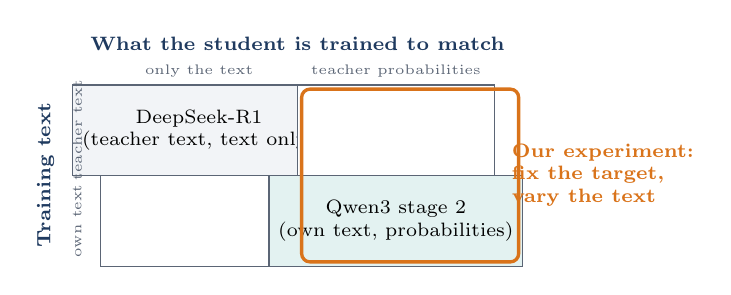
\begin{tikzpicture}[font=\scriptsize,
          cell/.style={draw=kdgray,minimum width=2.5cm,minimum height=1.15cm,align=center}]
        \node[cell,fill=kdlight] (a) at (0,0) {DeepSeek-R1\\(teacher text, text only)};
        \node[cell,fill=white] (b) at (2.5,0) {};
        \node[cell,fill=white] (c) at (0,-1.15) {};
        \node[cell,fill=kdteal!12] (d) at (2.5,-1.15) {Qwen3 stage 2\\(own text, probabilities)};
        \node[font=\scriptsize\bfseries,text=kdnavy] at (1.25,1.1) {What the student is trained to match};
        \node[font=\tiny,text=kdgray] at (0,0.75) {only the text};
        \node[font=\tiny,text=kdgray] at (2.5,0.75) {teacher probabilities};
        \node[font=\tiny,text=kdgray,rotate=90] at (-1.55,0) {teacher text};
        \node[font=\tiny,text=kdgray,rotate=90] at (-1.55,-1.15) {own text};
        \node[font=\scriptsize\bfseries,text=kdnavy,rotate=90] at (-1.95,-0.57) {Training text};
        % our experiment: fix the target, vary the text
        \draw[kdorange,very thick,rounded corners=3pt,visible on=<2->]
          ($(b.north west)+(0.06,-0.06)$) rectangle ($(d.south east)+(-0.06,0.06)$);
        \node[text=kdorange,font=\scriptsize\bfseries,align=left,anchor=west,visible on=<2->]
          at (3.85,-0.57) {Our experiment:\\fix the target,\\vary the text};
      \end{tikzpicture}
    \end{column}
    \begin{column}{0.42\textwidth}
      \small
      \begin{itemize}
        \item<1-> R1 changes \emph{both}: teacher text \emph{and} a
              text-only target.
        \item<1-> Qwen3 stage 2 uses the student's own text \emph{and}
              the full distribution.
        \item<2-> So which part helps? We keep the target fixed
              (the teacher's full next-token distribution) and change
              \textbf{only} where the training text comes from.
      \end{itemize}
    \end{column}
  \end{columns}
\end{frame}

% ------------------------------------------------------------------
\begin{frame}{Our research question\hfill\who{T3}}
  \begin{keybox}
    At an equal number of student updates, does the \textbf{source of the
    training text} (human-written, teacher-written, or the student's own)
    change how well \textbf{Qwen3-0.6B} learns from \textbf{Qwen3-4B}, when the
    target is always the teacher's full next-token distribution?
  \end{keybox}
  \vspace{0.2cm}
  \begin{columns}[T]
    \begin{column}{0.48\textwidth}
      \small
      \textbf{Why it could matter}
      \begin{itemize}
        \item<2-> Text written by others never contains the student's own
              mistakes, so it never learns what to do after one
              (\emph{exposure bias}, part 3).
        \item<3-> On-policy text fixes that, but costs about 10$\times$ more
              compute per step in our setup.
      \end{itemize}
    \end{column}
    \begin{column}{0.48\textwidth}
      \small
      \textbf{Plus the classic B3 question}
      \begin{itemize}
        \item<4-> Same human text, two targets: the teacher's
              probabilities vs hard labels (the correct token only).
        \item<5-> Tells us what the soft targets themselves are worth
              \src{Hinton et al., 2015}.
      \end{itemize}
    \end{column}
  \end{columns}
  \vspace{0.15cm}
  \begin{uncoverenv}<6->
  \begin{todobox}{T3's opening hook}
    Optional: a one-line real-world example of why small models matter
    (phone, cost per answer). Delete this box if not needed.
  \end{todobox}
  \end{uncoverenv}
\end{frame}

% =====================================================================
% 02-kd-basics.tex -- Distillation basics.  T2, 8 min
% Sources: Hinton et al. 2015 and Furlanello et al. 2018 (seed papers),
%          Kim & Rush 2016; notes/emre-notes-on-sources.txt (Mansourian
%          survey summary). Theory note: notes/theory/t2-soft-targets-temperature.md
% =====================================================================
\renewcommand{\sectioninfo}{Presenter: T2 \quad $\cdot$ \quad 8 minutes}
\section{Distillation basics}

% ------------------------------------------------------------------
\begin{frame}{Soft targets carry more than the right answer\hfill\est\ \who{T2}}
  \begin{columns}[c]
    \begin{column}{0.46\textwidth}
      \small
      \begin{itemize}
        \item<1-> \textbf{Hard label}: only the correct next token counts
              (one-hot).
        \item<1-> \textbf{Soft target}: the teacher's probability for
              \emph{every} token, including the wrong ones.
        \item<2-> Which wrong answers look almost right is information:
              Hinton calls it \emph{dark knowledge}.
        \item<3-> A temperature $T$ softens the distribution and makes
              that information visible:
              \[
                p_i(T) = \frac{\exp(z_i/T)}{\sum_j \exp(z_j/T)}
              \]
      \end{itemize}
      \vspace{-0.15cm}
      \src{Hinton, Vinyals and Dean, 2015}
    \end{column}
    \begin{column}{0.52\textwidth}
      \centering
      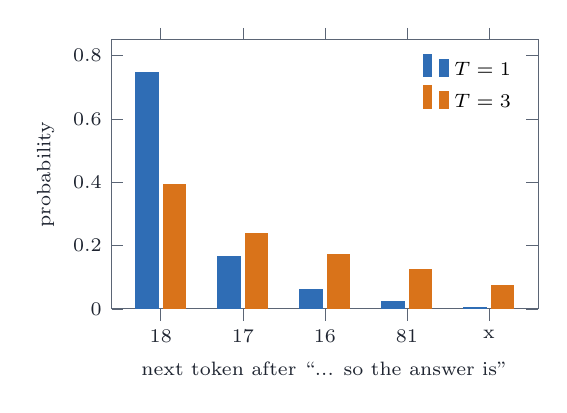
\begin{tikzpicture}
        \begin{axis}[kdaxis,
            width=7.0cm,height=5.0cm,
            ybar,bar width=8pt,
            ymin=0,ymax=0.85,
            symbolic x coords={a,b,c,d,e},
            xtick=data,
            xticklabels={18,17,16,81,x},
            ylabel={probability},
            xlabel={next token after ``... so the answer is''},
            legend pos=north east,
            legend cell align=left,
            enlarge x limits=0.15]
          \addplot[fill=kdblue,draw=kdblue] coordinates
            {(a,0.745) (b,0.166) (c,0.061) (d,0.023) (e,0.005)};
          \addplot[fill=kdorange,draw=kdorange,visible on=<3->] coordinates
            {(a,0.393) (b,0.239) (c,0.171) (d,0.123) (e,0.074)};
          \legend{$T=1$, $T=3$}
        \end{axis}
      \end{tikzpicture}

      {\tiny\color{kdgray} Illustration with made-up logits $z=(4.0,\,2.5,\,1.5,\,0.5,\,-1.0)$.}
    \end{column}
  \end{columns}
\end{frame}

% ------------------------------------------------------------------
\begin{frame}{The distillation loss\hfill\est\ \who{T2}}
  \begin{columns}[T]
    \begin{column}{0.55\textwidth}
      \small
      Match the student's distribution $p_S$ to the teacher's $p_T$ with
      the Kullback--Leibler divergence, token by token:
      \[
        \mathcal{L} \;=\; T^2 \cdot \mathrm{KL}\!\left(p_T^{(T)} \,\middle\|\, p_S^{(T)}\right)
        \;=\; T^2 \sum_{v} p_T^{(T)}(v)\,\log\frac{p_T^{(T)}(v)}{p_S^{(T)}(v)}
      \]
      \begin{itemize}
        \item<2-> The $T^2$ factor keeps the gradient size comparable
              across temperatures \src{Hinton et al., 2015}.
        \item<3-> Classic KD often mixes in a hard-label term; we use the
              soft target alone, so the arms differ only in their text.
        \item<4-> \textbf{Our setting}: $T = 1$ for every arm (not swept;
              see limitations).
      \end{itemize}
    \end{column}
    \begin{column}{0.42\textwidth}
      \begin{block}{In our experiment}
        \footnotesize
        \arm{human} and \arm{ref\_hardlabel} train on the \emph{same}
        cleaned GSM8K solutions:
        \begin{itemize}
          \item \arm{human}: forward KL to the teacher's distribution
          \item \arm{ref\_hardlabel}: cross-entropy on the correct token
        \end{itemize}
        The difference between them measures what the soft targets add
        (results, part 7).
      \end{block}
    \end{column}
  \end{columns}
\end{frame}

% ------------------------------------------------------------------
\begin{frame}{Two seed papers, two ideas we build on\hfill\est\ \who{T2}}
  \begin{columns}[T]
    \begin{column}{0.48\textwidth}
      \begin{block}{Born-Again Networks \src{Furlanello et al., 2018}}
        \footnotesize
        A student with the \emph{same} architecture as its teacher, trained
        on the teacher's soft outputs, can end up \emph{better} than the
        teacher. Distillation is more than compression: the gain comes from
        the soft targets, not from the teacher being bigger.
      \end{block}
    \end{column}
    \begin{column}{0.48\textwidth}
      \begin{block}{Sequence-level KD \src{Kim and Rush, 2016}}
        \footnotesize
        Instead of matching the teacher token by token on fixed text, train
        the student on whole sequences the \emph{teacher} wrote. In practice:
        generate teacher answers once, fine-tune on them. This is our
        \arm{teacher} arm, and the DeepSeek-R1 recipe.
      \end{block}
    \end{column}
  \end{columns}
  \vspace{0.2cm}
  \begin{todobox}{T2's own examples (theory note is still empty)}
    Fill \repofile{notes/theory/t2-soft-targets-temperature.md} and add here, if
    useful: a real teacher distribution for one GSM8K token from our
    teacher, and a one-sentence take-away for the audience.
  \end{todobox}
\end{frame}

% =====================================================================
% 03-kl-onpolicy.tex -- KL directions, on-policy training, exposure bias.
% T1, 6 min. Sources: src/kd/losses.py docstrings, Gu et al. 2024 (MiniLLM),
% Agarwal et al. 2024 (GKD), Bengio et al. 2015, Song & Zheng 2026 summary
% in notes/emre-notes-on-sources.txt.
% Theory note: notes/theory/t1-kl-directions-exposure-bias.md
% =====================================================================
\renewcommand{\sectioninfo}{Presenter: T1 \quad $\cdot$ \quad 6 minutes}
\section{KL directions and on-policy training}

% ------------------------------------------------------------------
\begin{frame}{Which way round? Forward vs reverse KL\hfill\est\ \who{T1}}
  \begin{columns}[c]
    \begin{column}{0.47\textwidth}
      \small
      \textbf{Forward KL} $\;\mathrm{KL}(p_T \,\|\, p_S)$: mass-covering.
      The student must put probability wherever the teacher does.
      \vspace{0.15cm}

      \uncover<3->{\textbf{Reverse KL} $\;\mathrm{KL}(p_S \,\|\, p_T)$:
      mode-seeking. The student is punished for mass where the teacher
      has little, so it commits to one mode \src{Gu et al., 2024}.}
      \vspace{0.15cm}

      \begin{uncoverenv}<4->
      \begin{keybox}
        \footnotesize We use \textbf{forward KL} for all four main arms, the
        classic distillation target. Reverse KL on \arm{onpolicy} was a
        stretch run and was not done.
      \end{keybox}
      \end{uncoverenv}
    \end{column}
    \begin{column}{0.50\textwidth}
      \centering
      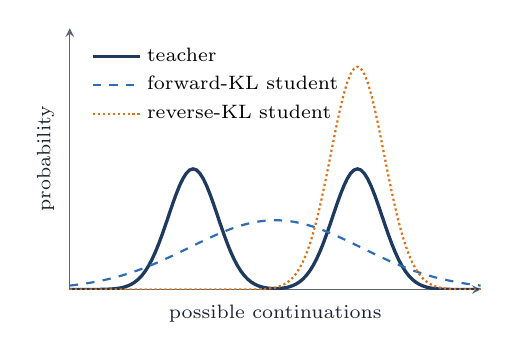
\begin{tikzpicture}
        \begin{axis}[kdaxis,width=6.8cm,height=4.9cm,
            domain=-5:5,samples=121,ymin=0,ymax=0.72,
            axis lines=left,xtick=\empty,ytick=\empty,
            xlabel={possible continuations},ylabel={probability},
            legend pos=north west,legend cell align=left]
          \addplot[kdnavy,very thick] {0.5*exp(((x+2)*(x+2))/(-0.72))/(0.6*sqrt(2*pi))
                                     + 0.5*exp(((x-2)*(x-2))/(-0.72))/(0.6*sqrt(2*pi))};
          \addplot[kdblue,thick,dashed,visible on=<2->] {exp((x*x)/(-8.72))/(2.09*sqrt(2*pi))};
          \addplot[kdorange,thick,densely dotted,visible on=<3->] {exp(((x-2)*(x-2))/(-0.845))/(0.65*sqrt(2*pi))};
          \legend{teacher, forward-KL student, reverse-KL student}
        \end{axis}
      \end{tikzpicture}

      {\tiny\color{kdgray} Illustration: a two-mode teacher and the best single-mode student under each divergence.}
    \end{column}
  \end{columns}
\end{frame}

% ------------------------------------------------------------------
\begin{frame}{Exposure bias: practising on someone else's text\hfill\est\ \who{T1}}
  \centering
  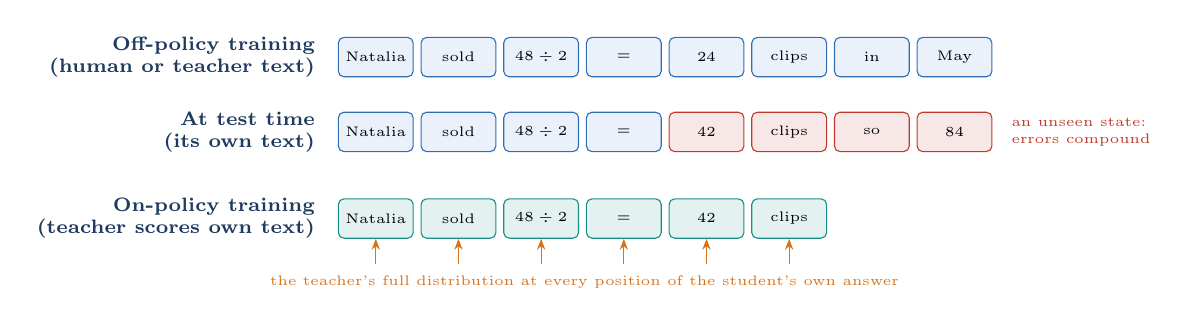
\begin{tikzpicture}[font=\tiny,
      tok/.style={draw=kdgray,rounded corners=2pt,minimum width=0.95cm,minimum height=0.5cm,fill=white,inner sep=1.5pt},
      good/.style={tok,fill=kdpale,draw=kdblue},
      bad/.style={tok,fill=kdred!12,draw=kdred},
      own/.style={tok,fill=kdteal!12,draw=kdteal}]
    % row 1: off-policy training
    \node[anchor=east,align=right,text=kdnavy,font=\scriptsize\bfseries] at (-0.1,0) {Off-policy training\\(human or teacher text)};
    \foreach \i/\w in {0/Natalia,1/sold,2/$48\div2$,3/=,4/24,5/clips,6/in,7/May}
      \node[good] at (\i*1.05+0.55,0) {\w};
    % row 2: test time, the student's own prefix
    \node[anchor=east,align=right,text=kdnavy,font=\scriptsize\bfseries,visible on=<2->] at (-0.1,-0.95) {At test time\\(its own text)};
    \foreach \i/\w in {0/Natalia,1/sold,2/$48\div2$,3/=}
      \node[good,visible on=<2->] at (\i*1.05+0.55,-0.95) {\w};
    \node[bad,visible on=<2->] at (4*1.05+0.55,-0.95) {42};
    \foreach \i/\w in {5/clips,6/so,7/84}
      \node[bad,visible on=<3->] at (\i*1.05+0.55,-0.95) {\w};
    \node[text=kdred,font=\tiny,align=left,visible on=<3->,anchor=west] at (8.5,-0.95) {an unseen state:\\errors compound};
    % row 3: on-policy training
    \node[anchor=east,align=right,text=kdnavy,font=\scriptsize\bfseries,visible on=<4->] at (-0.1,-2.05) {On-policy training\\(teacher scores own text)};
    \foreach \i/\w in {0/Natalia,1/sold,2/$48\div2$,3/=,4/42,5/clips}
      \node[own,visible on=<4->] (o\i) at (\i*1.05+0.55,-2.05) {\w};
    \foreach \i in {0,...,5}
      \draw[-{Stealth[length=1.4mm]},kdorange,visible on=<4->] ($(o\i.south)+(0,-0.32)$) -- (o\i.south);
    \node[text=kdorange,font=\tiny,anchor=north,visible on=<4->] at (3.2,-2.65) {the teacher's full distribution at every position of the student's own answer};
  \end{tikzpicture}
  \vspace{0.1cm}
  \begin{itemize}\small
    \item<2-> Off-policy training only ever shows \emph{correct} prefixes; the student
          never learns to recover from its own mistakes \src{Bengio et al., 2015}.
    \item<4-> On-policy distillation trains on the student's own prefixes, with dense
          token-level feedback from the teacher \src{Agarwal et al., 2024}.
  \end{itemize}
\end{frame}

% ------------------------------------------------------------------
\begin{frame}{Why on-policy should help, and what it costs\hfill\est\ \who{T1}}
  \begin{columns}[T]
    \begin{column}{0.48\textwidth}
      \begin{block}{The argument}
        \footnotesize
        \begin{itemize}
          \item Imitation learning: off-policy error can grow with the
                \emph{square} of the sequence length, on-policy only
                linearly (DAgger, Ross et al., 2011).
          \item GKD unifies the methods: choose \emph{whose} text is
                sampled and \emph{which} divergence is used
                \src{Agarwal et al., 2024}.
          \item Survey advice: off-policy is enough for style and
                knowledge; on-policy pays off for reasoning
                \src{Song and Zheng, 2026}.
        \end{itemize}
      \end{block}
    \end{column}
    \begin{column}{0.48\textwidth}
      \begin{block}{The cost, in our own runs \ours}
        \footnotesize
        Training time per run, seed 2 / seed 3, on Kaggle T4 x2:
        \begin{itemize}
          \item \arm{onpolicy}: 3.34 / 3.01 GPU-hours
          \item the other arms: 0.21 to 0.36 GPU-hours
        \end{itemize}
        About 10$\times$ more, because the student writes 4 new answers
        at every step (about 85 to 90\% of the step time).
      \end{block}
    \end{column}
  \end{columns}
  \vspace{0.15cm}
  \begin{todobox}{T1's own explanation (theory note is still empty)}
    Fill \repofile{notes/theory/t1-kl-directions-exposure-bias.md}; check the
    DAgger and survey claims against the papers before presenting.
  \end{todobox}
\end{frame}

% =====================================================================
% 04-literature.tex -- What the literature establishes.  E2, 8 min
% Sources: Sources/README.md (literature table), report/references.bib,
%          notes/emre-notes-on-sources.txt.
% Theory note: notes/theory/e2-literature-map-gsm8k-grading.md
% Rule from the brief: group papers by the question they answer, do not
% present one paper per slide.
% =====================================================================
\renewcommand{\sectioninfo}{Presenter: E2 \quad $\cdot$ \quad 8 minutes}
\section{What the literature establishes}

% ------------------------------------------------------------------
\begin{frame}{Five questions, and what is known about each\hfill\est\ \who{E2}}
  \scriptsize
  \renewcommand{\arraystretch}{1.25}
  \begin{tabular}{@{}>{\raggedright\arraybackslash}p{2.8cm}>{\raggedright\arraybackslash}p{4.0cm}>{\raggedright\arraybackslash}p{6.2cm}@{}}
    \toprule
    \textbf{Question} & \textbf{Key sources} & \textbf{What they establish} \\
    \midrule
    \uncover<1->{Do soft targets help?} & \uncover<1->{Hinton et al. 2015; Furlanello et al. 2018}
      & \uncover<1->{Teacher probabilities carry information beyond the label; a same-size student can even beat its teacher.} \\
    \uncover<2->{Can a student learn from teacher text alone?} & \uncover<2->{Kim and Rush 2016; DeepSeek-AI 2025}
      & \uncover<2->{Yes: training on teacher-written sequences works, up to large reasoning models.} \\
    \uncover<3->{Does training on its own text help?} & \uncover<3->{Agarwal et al. 2024 (GKD); Gu et al. 2024 (MiniLLM); Qwen Team 2025; Lu and Thinking Machines 2025}
      & \uncover<3->{On-policy distillation beats off-policy on several tasks; the best divergence depends on the task.} \\
    \uncover<4->{Why could it help?} & \uncover<4->{Bengio et al. 2015; Ross et al. 2011}
      & \uncover<4->{Exposure bias: models trained only on correct prefixes compound their own errors.} \\
    \uncover<5->{How do we measure it fairly?} & \uncover<5->{Cobbe et al. 2021; Miller 2024; Stanton et al. 2021; Wu et al. 2025}
      & \uncover<5->{GSM8K is graded by its final number; scores need error bars and paired tests; fidelity is not accuracy; public benchmarks may be contaminated.} \\
    \bottomrule
  \end{tabular}
\end{frame}

% ------------------------------------------------------------------
\begin{frame}{What is still open, and where we fit\hfill\est\ \who{E2}}
  \begin{columns}[T]
    \begin{column}{0.5\textwidth}
      \begin{block}{Open points in the literature}
        \footnotesize
        \begin{itemize}
          \item On-policy distillation helps only when teacher and student
                ``think'' compatibly and the teacher knows something new;
                same-family pairs can look identical
                \src{Li et al., 2026}.
          \item Recommended recipe: off-policy warm-up, then on-policy
                \src{Song and Zheng, 2026}.
          \item Published comparisons change several things at once
                (data, target, compute), so the source of the text is
                rarely isolated.
        \end{itemize}
      \end{block}
    \end{column}
    \begin{column}{0.46\textwidth}
      \begin{block}{Our contribution}
        \footnotesize
        \begin{itemize}
          \item One target for every arm (forward KL to the teacher's full
                distribution).
          \item Equal updates, identical questions in identical order.
          \item A small, cheap setting: a 0.6B student, a 4B teacher,
                free Kaggle GPUs, three seeds.
          \item Checked that there is something to distil first
                (headroom test, part 5).
        \end{itemize}
      \end{block}
    \end{column}
  \end{columns}
  \vspace{0.15cm}
  \begin{todobox}{E2's literature map (theory note is still empty)}
    Fill \repofile{notes/theory/e2-literature-map-gsm8k-grading.md}. Verify every
    reference against the paper itself (the bib file says ``verify''); Ross et al.
    2011, Li et al. 2026 and Song and Zheng 2026 still need entries in
    \repofile{report/references.bib}.
  \end{todobox}
\end{frame}

% =====================================================================
% 05-design.tex -- Experiment design and pipeline.
% T3 4 min (pipeline, setup, settings, headroom), T2 2 min (arms, text),
% T1 4 min (fairness, on-policy step, loss).
% Sources: configs/default.yaml, src/kd/{data,train,losses}.py,
%          data/teacher_sequences.meta.json, results/runs/pilot_onpolicy_*,
%          notebooks/archive/headroom-test.ipynb
% =====================================================================
\renewcommand{\sectioninfo}{Presenters: T3 (4 min), T2 (2 min), T1 (4 min)}
\section{Experiment design and pipeline}

% ------------------------------------------------------------- T3
\begin{frame}{The whole pipeline, from question to slide\hfill\who{T3}}
  \centering
  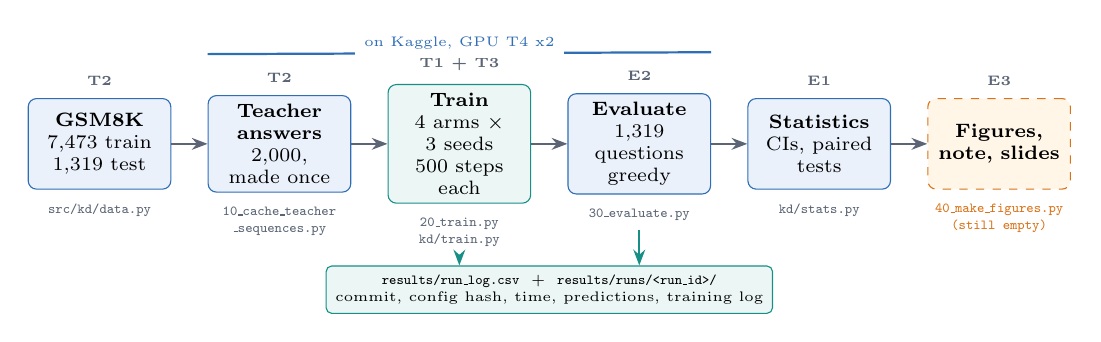
\begin{tikzpicture}[node distance=0.46cm,stage/.append style={text width=1.6cm}]
    \node[stage] (s1) {\textbf{GSM8K}\\7,473 train\\1,319 test};
    \node[stage,right=of s1,visible on=<2->] (s2) {\textbf{Teacher answers}\\2,000, made once};
    \node[stageT,right=of s2,visible on=<3->] (s3) {\textbf{Train}\\4 arms $\times$ 3 seeds\\500 steps each};
    \node[stage,right=of s3,visible on=<4->] (s4) {\textbf{Evaluate}\\1,319 questions\\greedy};
    \node[stage,right=of s4,visible on=<5->] (s5) {\textbf{Statistics}\\CIs, paired tests};
    \node[stageX,right=of s5,visible on=<6->] (s6) {\textbf{Figures, note, slides}};
    % arrows
    \draw[flow,visible on=<2->] (s1) -- (s2);
    \draw[flow,visible on=<3->] (s2) -- (s3);
    \draw[flow,visible on=<4->] (s3) -- (s4);
    \draw[flow,visible on=<5->] (s4) -- (s5);
    \draw[flow,visible on=<6->] (s5) -- (s6);
    % owners
    \tikzset{owner/.style={font=\tiny\bfseries,text=kdgray}}
    \node[owner,above=0.04cm of s1] {T2};
    \node[owner,above=0.04cm of s2,visible on=<2->] {T2};
    \node[owner,above=0.04cm of s3,visible on=<3->] {T1 + T3};
    \node[owner,above=0.04cm of s4,visible on=<4->] {E2};
    \node[owner,above=0.04cm of s5,visible on=<5->] {E1};
    \node[owner,above=0.04cm of s6,visible on=<6->] {E3};
    % files
    \node[filelabel,below=0.06cm of s1] {src/kd/data.py};
    \node[filelabel,below=0.06cm of s2,visible on=<2->] {10\_cache\_teacher\\\_sequences.py};
    \node[filelabel,below=0.06cm of s3,visible on=<3->] (f3) {20\_train.py\\kd/train.py};
    \node[filelabel,below=0.06cm of s4,visible on=<4->] (f4) {30\_evaluate.py};
    \node[filelabel,below=0.06cm of s5,visible on=<5->] {kd/stats.py};
    \node[filelabel,below=0.06cm of s6,visible on=<6->,text=kdorange] {40\_make\_figures.py\\(still empty)};
    % Kaggle bracket over the GPU stages
    \draw[kdblue,thick,visible on=<3->] ($(s2.north west)+(0,0.52)$) -- ($(s4.north east)+(0,0.52)$);
    \node[font=\tiny,text=kdblue,fill=white,visible on=<3->] at ($(s3.north)+(0,0.52)$) {on Kaggle, GPU T4 x2};
    % run log
    \node[draw=kdteal,fill=kdteal!8,rounded corners=2pt,font=\tiny,align=center,visible on=<4->] (log)
      at ($(s3.south)!0.5!(s4.south)+(0,-1.15)$)
      {\texttt{results/run\_log.csv} \;+\; \texttt{results/runs/<run\_id>/}\\
       commit, config hash, time, predictions, training log};
    \draw[flow,kdteal,visible on=<4->] (f3.south) -- (f3.south |- log.north);
    \draw[flow,kdteal,visible on=<4->] (f4.south) -- (f4.south |- log.north);
  \end{tikzpicture}
  \vspace{0.1cm}

  {\scriptsize Every step is a numbered script; the Kaggle notebook only clones the repo at a fixed commit and calls them.}
\end{frame}

% ------------------------------------------------------------------
\begin{frame}{Models, data and compute\hfill\who{T3}}
  \begin{columns}[T]
    \begin{column}{0.6\textwidth}
      \footnotesize
      \renewcommand{\arraystretch}{1.2}
      \begin{tabular}{@{}>{\bfseries}l>{\raggedright\arraybackslash}p{5.6cm}@{}}
        \toprule
        Teacher & Qwen3-4B, frozen, fp16 on GPU 1 (about 8 GB) \\
        Student & Qwen3-0.6B, all weights trained, fp32 weights with fp16
                  compute on GPU 0 (about 11 GB) \\
        Training data & a fixed pool of 2,000 GSM8K training questions \\
        Test data & all 1,319 GSM8K test questions \\
        Prompt & ``Solve the problem step by step. Put the final number
                 at the end.'' (thinking mode off) \\
        Updates & 500 steps of 4 questions; AdamW, learning rate
                  $5\cdot10^{-6}$, gradient clip 1.0 \\
        Seeds & 1, 2, 3: change the question order and the sampling \\
        Hardware & Kaggle, 2 $\times$ T4 (16 GB each), one free account per member \\
        \bottomrule
      \end{tabular}
    \end{column}
    \begin{column}{0.36\textwidth}
      \begin{block}{Why these models}
        \footnotesize
        \begin{itemize}
          \item Largest pair that fits on free Kaggle GPUs: teacher
                (8 GB) and training student (11 GB) need one T4 each.
          \item Same family: one tokenizer and vocabulary, so the
                distributions can be compared token by token.
          \item GSM8K: graded automatically by the final number.
        \end{itemize}
      \end{block}
    \end{column}
  \end{columns}
\end{frame}

% ------------------------------------------------------------------
\begin{frame}[fragile]{Settings we locked, and why\hfill\ours\ \who{T3}}
  \begin{columns}[T]
    \begin{column}{0.53\textwidth}
\begin{lstlisting}[style=kdplain]
# configs/default.yaml  (commit f2accc6)
data:
  pool_size: 2000         # fixed questions
train:
  questions_per_step: 4   # 500 steps
  lr: 5.0e-6              # pilot sweep
  loss: forward_kl        # hard-label: cross-entropy
  temperature: 1.0        # distillation T
  oom_retries: 2          # retry, never skip
generation:
  max_new_tokens: 512     # 384 cut 14% of teacher
  sampling: {temperature: 0.7, top_p: 0.8, top_k: 20}
\end{lstlisting}
      {\tiny\color{kdgray} Config hash of every main run: \texttt{85bee6cac023}}
    \end{column}
    \begin{column}{0.44\textwidth}
      \footnotesize
      \textbf{Pilot sweep}: on-policy arm, seed 1, 100 steps, accuracy
      on all 1,319 test questions.
      \vspace{0.1cm}

      \centering
      \begin{tabular}{@{}lr@{\qquad}lr@{}}
        \toprule
        lr & acc.\ \% & sampling $T$ & acc.\ \% \\
        \midrule
        $5\cdot10^{-6}$ & \textbf{65.6} & 0.5 & 64.5 \\
        $1\cdot10^{-5}$ & 60.6 & \textbf{0.7} & \textbf{65.6} \\
        $2\cdot10^{-5}$ & 50.2 & 1.0 & 63.5 \\
        \bottomrule
      \end{tabular}

      \raggedright
      \vspace{0.15cm}
      Larger steps pulled the already tuned student away from what it did
      well. Caveat: chosen on the on-policy arm and on the test set
      (see limitations).
    \end{column}
  \end{columns}
\end{frame}

% ------------------------------------------------------------------
\begin{frame}{Is there anything to distil? The headroom test\hfill\ours\ \who{T3}}
  \begin{columns}[c]
    \begin{column}{0.45\textwidth}
      \centering
      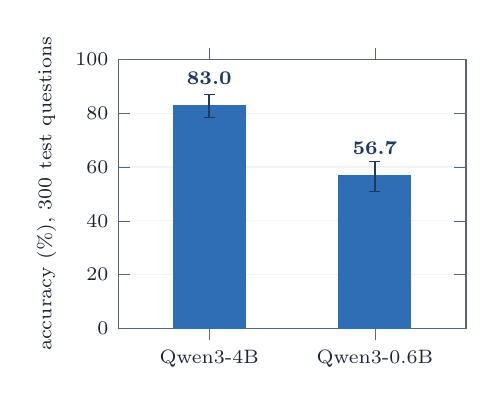
\begin{tikzpicture}
        \begin{axis}[kdaxis,width=6.0cm,height=5.0cm,
            ybar,bar width=26pt,ymin=0,ymax=100,
            symbolic x coords={teacher,student},xtick=data,
            xticklabels={Qwen3-4B,Qwen3-0.6B},
            ylabel={accuracy (\%), 300 test questions},
            enlarge x limits=0.55,ymajorgrids]
          \addplot[fill=kdblue,draw=kdblue,
              error bars/.cd,y dir=both,y explicit,error bar style={kdnavy,thick}]
            coordinates {(teacher,83.0) +=(0,3.8) -=(0,4.7)
                         (student,56.7) +=(0,5.5) -=(0,5.7)};
          \node[font=\scriptsize\bfseries,text=kdnavy] at (axis cs:teacher,93) {83.0};
          \node[font=\scriptsize\bfseries,text=kdnavy] at (axis cs:student,67) {56.7};
        \end{axis}
      \end{tikzpicture}
    \end{column}
    \begin{column}{0.52\textwidth}
      \small
      \begin{itemize}
        \item Before training anything: are the two models far enough apart?
        \item Zero-shot, greedy, the same 300 random test questions,
              95\% Wilson intervals.
        \item Paired gap: \textbf{+26.3 points}, bootstrap 95\% CI
              [21.0, 31.7]. Rule agreed in advance: proceed if the gap is at
              least 10 points and the CI excludes 0.
        \item On all 1,319 questions with 512 tokens the untrained student
              scores \textbf{62.0\%} [59.4, 64.6]: our real baseline.
      \end{itemize}
      \begin{todobox}{Teacher on the full test set (E2)}
        \arm{ref\_teacher} is still \emph{planned} in the run log. Its accuracy
        on all 1,319 questions replaces the 300-question number here.
      \end{todobox}
    \end{column}
  \end{columns}
\end{frame}

% ------------------------------------------------------------- T2
\begin{frame}{Four arms, one difference\hfill\who{T2}}
  \small
  \renewcommand{\arraystretch}{1.25}
  \begin{tabular}{@{}l>{\raggedright\arraybackslash}p{4.0cm}>{\raggedright\arraybackslash}p{3.8cm}l@{}}
    \toprule
    \textbf{Arm} & \textbf{Training text} & \textbf{Target} & \textbf{Teacher model} \\
    \midrule
    \uncover<1->{\arm{human}} & \uncover<1->{cleaned GSM8K solutions} & \uncover<1->{forward KL to the teacher} & \uncover<1->{needed} \\
    \uncover<2->{\arm{teacher}} & \uncover<2->{teacher answers, generated once (greedy)} & \uncover<2->{forward KL to the teacher} & \uncover<2->{needed} \\
    \uncover<3->{\arm{onpolicy}} & \uncover<3->{the student's own answers, new at every step} & \uncover<3->{forward KL to the teacher} & \uncover<3->{needed} \\
    \uncover<4->{\arm{ref\_hardlabel}} & \uncover<4->{cleaned GSM8K solutions} & \uncover<4->{cross-entropy on the correct token} & \uncover<4->{not used} \\
    \midrule
    \uncover<5->{\arm{ref\_student0}} & \multicolumn{3}{l}{\uncover<5->{reference: the untrained student, evaluated once}} \\
    \uncover<5->{\arm{ref\_teacher}} & \multicolumn{3}{l}{\uncover<5->{reference: the teacher itself \textcolor{kdorange}{(not evaluated yet)}}} \\
    \bottomrule
  \end{tabular}
  \vspace{0.25cm}
  \begin{uncoverenv}<6->
  \begin{keybox}
    \footnotesize Identical in every arm: the 2,000 questions, their order, 500 steps, optimizer,
    learning rate, maximum length. The \textbf{only} difference is the training text
    (and the target, for the hard-label reference).
  \end{keybox}
  \end{uncoverenv}
\end{frame}

% ------------------------------------------------------------------
\begin{frame}[fragile]{Building the training text\hfill\who{T2}}
  \begin{columns}[T]
    \begin{column}{0.48\textwidth}
      \scriptsize\textbf{Raw GSM8K solution}
\begin{lstlisting}[style=kdplain]
Natalia sold 48/2 = <<48/2=24>>24 clips in May.
Natalia sold 48+24 = <<48+24=72>>72 clips
altogether in April and May.
#### 72
\end{lstlisting}
      \scriptsize\textbf{After \texttt{clean\_solution()}} (\repofile{src/kd/data.py})
\begin{lstlisting}[style=kdplain]
Natalia sold 48/2 = 24 clips in May.
Natalia sold 48+24 = 72 clips
altogether in April and May.
The final answer is 72.
\end{lstlisting}
      \tiny Calculator notes removed; the last number is always the answer,
      so the grading rule marks every cleaned solution correct.
    \end{column}
    \begin{column}{0.48\textwidth}
      \begin{block}{Teacher answers \ours}
        \footnotesize
        \begin{itemize}
          \item Generated once for all 2,000 pool questions, greedy,
                512 tokens, not filtered for correctness
          \item 92.1\% correct, mean 260 tokens, 2\% cut off
          \item About 1.5 hours on one Kaggle session; committed as
                \repofile{data/teacher\_sequences.jsonl}
        \end{itemize}
      \end{block}
      \begin{block}{On-policy answers}
        \footnotesize
        The student samples 4 new answers at every step
        (temperature 0.7, top-p 0.8, top-k 20), so this text changes as
        the student learns.
      \end{block}
    \end{column}
  \end{columns}
\end{frame}

% ------------------------------------------------------------- T1
\begin{frame}[fragile]{Equal updates: keeping the arms fair\hfill\who{T1}}
  \begin{columns}[T]
    \begin{column}{0.55\textwidth}
\begin{lstlisting}
def question_order(question_ids, seed, epochs=1):
    """The order of the pool: depends ONLY on the seed."""
    # own generator, untouched by on-policy sampling
    rng = random.Random(f"data-order:{seed}")
    order = []
    for _ in range(epochs):
        ids = sorted(question_ids)
        rng.shuffle(ids)
        order.extend(ids)
    return order

def question_ids_hash(question_ids):
    """Fingerprint of one step; must match across arms."""
    return hashlib.sha256(
        ",".join(question_ids).encode()).hexdigest()[:16]
\end{lstlisting}
      {\tiny\color{kdgray} From \texttt{src/kd/train.py}}
    \end{column}
    \begin{column}{0.42\textwidth}
      \footnotesize
      Two bugs in our first notebook made the comparison unfair:
      \begin{enumerate}
        \item<2-> \textbf{Shared randomness}: one global generator set the
              order \emph{and} the sampling, so arms saw different orders.
              Now each has its own generator.
        \item<3-> \textbf{Skipped steps}: an out-of-memory error skipped a
              step. Now the same step is retried, and the run stops after
              two failures.
      \end{enumerate}
      \begin{uncoverenv}<4->
      \begin{block}{Checked on our runs \ours}
        \scriptsize Seeds 2 and 3: identical question hashes in all four arms
        at all 500 steps, 0 skipped steps (\texttt{fairness\_check} in
        \repofile{kd/stats.py}).
      \end{block}
      \end{uncoverenv}
    \end{column}
  \end{columns}
\end{frame}

% ------------------------------------------------------------------
\begin{frame}{One on-policy training step\hfill\who{T1}}
  \centering
  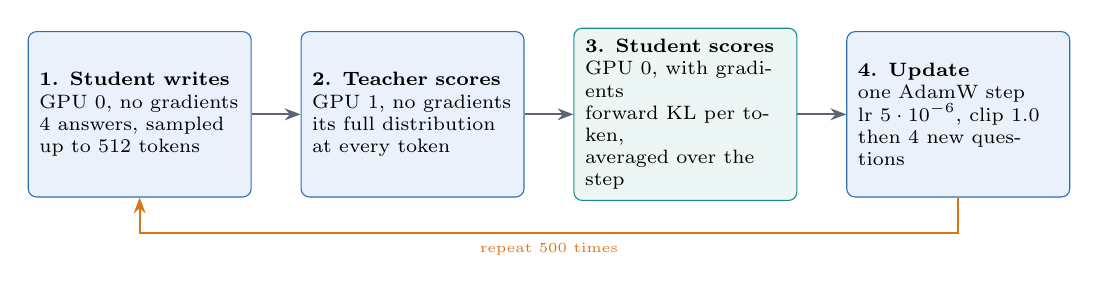
\begin{tikzpicture}[node distance=0.62cm,
      box/.style={draw=kdblue,fill=kdpale,rounded corners=3pt,align=left,
                  font=\scriptsize,text width=2.55cm,minimum height=2.1cm,inner sep=4pt}]
    \node[box] (a) {\textbf{1. Student writes}\\GPU 0, no gradients\\4 answers, sampled\\up to 512 tokens};
    \node[box,right=of a,visible on=<2->] (b) {\textbf{2. Teacher scores}\\GPU 1, no gradients\\its full distribution\\at every token};
    \node[box,right=of b,visible on=<3->,draw=kdteal,fill=kdteal!8] (c) {\textbf{3. Student scores}\\GPU 0, with gradients\\forward KL per token,\\averaged over the step};
    \node[box,right=of c,visible on=<4->] (d) {\textbf{4. Update}\\one AdamW step\\lr $5\cdot10^{-6}$, clip 1.0\\then 4 new questions};
    \draw[flow,visible on=<2->] (a) -- (b);
    \draw[flow,visible on=<3->] (b) -- (c);
    \draw[flow,visible on=<4->] (c) -- (d);
    \draw[flow,kdorange,visible on=<5->] (d.south) -- ++(0,-0.45) -| (a.south)
      node[pos=0.25,below,font=\tiny,text=kdorange] {repeat 500 times};
  \end{tikzpicture}
  \vspace{0.3cm}

  \small
  \begin{itemize}
    \item<5-> The other arms skip step 1: their text is fixed (a cleaned solution
          or a cached teacher answer). Steps 2 to 4 are identical.
    \item<6-> Step 1 takes most of the time: 18.8 to 21.5 of the 21.5 to 23.9
          seconds per on-policy step (87 to 90\%), against 1.5 to 2.3 seconds
          per step for the other arms \ours.
  \end{itemize}
\end{frame}

% ------------------------------------------------------------------
\begin{frame}[fragile]{The loss in code\hfill\who{T1}}
\begin{lstlisting}
def forward_kl(student_logits, teacher_logits, temperature=1.0):
    """KL(teacher || student) per token: the classic distillation target."""
    log_p_s = F.log_softmax(student_logits.float() / temperature, dim=-1)
    log_p_t = F.log_softmax(teacher_logits.float() / temperature, dim=-1)
    return (log_p_t.exp() * (log_p_t - log_p_s)).sum(dim=-1)

# inside distillation_loss(): only answer tokens count
s_logits, targets = response_positions(student_logits, input_ids, response_mask)
per_token = forward_kl(s_logits, t_logits, temperature) * temperature ** 2
return per_token.sum() / normalizer   # average over every answer token of the step
\end{lstlisting}
  {\tiny\color{kdgray} From \texttt{src/kd/losses.py}}
  \vspace{0.1cm}

  \begin{columns}[T]
    \begin{column}{0.32\textwidth}
      \footnotesize\textbf{Alignment.} Logits at position $t$ predict token
      $t+1$; getting this wrong is the most common silent bug.
    \end{column}
    \begin{column}{0.32\textwidth}
      \footnotesize\textbf{Masking.} Prompt and padding never count; the
      average runs over all answer tokens of the step.
    \end{column}
    \begin{column}{0.32\textwidth}
      \footnotesize\textbf{Tested.} KL is 0 for identical logits, matches
      \texttt{torch}'s \texttt{kl\_div}, ignores masked positions
      (10 tests).
    \end{column}
  \end{columns}
\end{frame}

% =====================================================================
% 06-evaluation.tex -- Evaluation method.  E2 2 min (grading), E1 2 min (statistics)
% Sources: src/kd/answer_extraction.py, src/kd/evaluate.py,
%          scripts/30_evaluate.py, src/kd/stats.py,
%          notes/theory/e1-fair-evaluation-statistics.md
% =====================================================================
\renewcommand{\sectioninfo}{Presenters: E2 (2 min), E1 (2 min)}
\section{Evaluation method}

% ------------------------------------------------------------- E2
\begin{frame}[fragile]{Grading an answer\hfill\who{E2}}
  \begin{columns}[T]
    \begin{column}{0.55\textwidth}
\begin{lstlisting}
def extract_last_number(text):
    """The model's answer: the last number it wrote."""
    cleaned = text.replace(",", "").replace("$", "")
    numbers = re.findall(r"-?\d+(?:\.\d+)?", cleaned)
    return float(numbers[-1]) if numbers else None

# correct if it equals the gold answer after "####"
is_correct = (predicted is not None
              and abs(predicted - expected) < 1e-6)
\end{lstlisting}
      {\tiny\color{kdgray} From \texttt{src/kd/answer\_extraction.py} and \texttt{src/kd/evaluate.py} (shortened)}
    \end{column}
    \begin{column}{0.42\textwidth}
      \footnotesize
      \begin{itemize}
        \item All \textbf{1,319} GSM8K test questions, the same prompt for
              every model, thinking mode off.
        \item \textbf{Greedy} decoding, batched, at most \textbf{512} new
              tokens; an answer without an end token is flagged as cut off.
        \item One file per run: \repofile{predictions.jsonl}, one line per
              question.
      \end{itemize}
      \begin{block}{Example}
        \scriptsize
        Model: ``\dots she makes \$18 every day.'' $\rightarrow$ 18.0\\
        Gold: ``\dots\ \#\#\#\# 18'' $\rightarrow$ 18.0 \quad \textcolor{kdteal}{\textbf{correct}}
      \end{block}
    \end{column}
  \end{columns}
\end{frame}

% ------------------------------------------------------------- E1
\begin{frame}{Error bars and fair comparisons\hfill\est\ \who{E1}}
  \begin{columns}[T]
    \begin{column}{0.5\textwidth}
      \small
      \textbf{One accuracy}: a 95\% Wilson interval for $k$ correct out of
      $n$, with $p = k/n$ and $z = 1.96$:
      \[
        \frac{p + \frac{z^2}{2n} \pm z\sqrt{\frac{p(1-p)}{n} + \frac{z^2}{4n^2}}}{1 + \frac{z^2}{n}}
      \]
      It stays inside $[0,1]$ and behaves near 0\% and 100\%
      \src{Wilson, 1927; Brown et al., 2001}.
    \end{column}
    \begin{column}{0.47\textwidth}
      \small
      \uncover<2->{\textbf{Two runs}: they answered the \emph{same} questions,
      so compare question by question:
      \[ d = \tfrac{1}{n}\textstyle\sum_i (a_i - b_i), \quad a_i, b_i \in \{0,1\} \]
      Resample the questions 10,000 times (seed 42) and take the 2.5\% and
      97.5\% points of $d$: the paired bootstrap interval
      \src{Miller, 2024; Efron and Tibshirani, 1993}.}
    \end{column}
  \end{columns}
  \vspace{0.2cm}
  \begin{uncoverenv}<3->
  \begin{keybox}
    \footnotesize \textbf{Rules we follow.} The bootstrap covers the choice of test
    questions, not training noise, so every seed is shown separately with its
    mean and range. We never pick the best seed. A difference whose interval
    contains 0 is ``no detectable difference''.
  \end{keybox}
  \end{uncoverenv}
\end{frame}

% =====================================================================
% 07-results.tex -- Results.  E1 6 min (accuracy, seeds, differences),
% E3 4 min (cost, length, size and speed)
%
% Numbers: python -m kd.stats (src/kd/stats.py, E1) on results/runs/,
% seeds 2 and 3 plus ref_student0, computed on Nov 25.
% When seed 1 and ref_teacher arrive: rerun kd.stats and update the
% coordinates below (or replace the charts with the PNGs from
% scripts/40_make_figures.py once E3 has written it).
% =====================================================================
\renewcommand{\sectioninfo}{Presenters: E1 (6 min), E3 (4 min)}
\section{Results}

% ------------------------------------------------------------- E1
\begin{frame}{On-policy text beats every other source\hfill\ours\ \who{E1}}
  \begin{columns}[c]
    \begin{column}{0.6\textwidth}
      \centering
      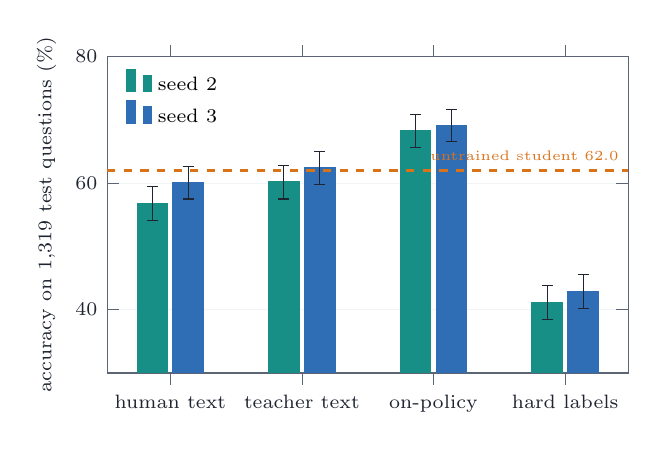
\begin{tikzpicture}
        \begin{axis}[kdaxis,width=8.2cm,height=5.6cm,
            ybar,bar width=11pt,ymin=30,ymax=80,
            symbolic x coords={human,teacher,onpolicy,hardlabel},xtick=data,
            xticklabels={human text,teacher text,on-policy,hard labels},
            ylabel={accuracy on 1,319 test questions (\%)},
            enlarge x limits=0.16,ymajorgrids,
            legend style={at={(0.02,0.98)},anchor=north west},legend cell align=left]
          \addplot[fill=kdteal,draw=kdteal,
              error bars/.cd,y dir=both,y explicit,error bar style={kdink}]
            coordinates {(human,56.8) +=(0,2.6) -=(0,2.7)
                         (teacher,60.2) +=(0,2.6) -=(0,2.7)
                         (onpolicy,68.3) +=(0,2.5) -=(0,2.6)
                         (hardlabel,41.2) +=(0,2.6) -=(0,2.7)};
          \addplot[fill=kdblue,draw=kdblue,
              error bars/.cd,y dir=both,y explicit,error bar style={kdink}]
            coordinates {(human,60.1) +=(0,2.6) -=(0,2.6)
                         (teacher,62.5) +=(0,2.5) -=(0,2.7)
                         (onpolicy,69.1) +=(0,2.5) -=(0,2.5)
                         (hardlabel,42.8) +=(0,2.7) -=(0,2.6)};
          \draw[kdorange,thick,dashed] (rel axis cs:0,0.64) -- (rel axis cs:1,0.64);
          \node[font=\tiny,text=kdorange,anchor=south east] at (rel axis cs:1,0.64) {untrained student 62.0};
          \legend{seed 2, seed 3}
        \end{axis}
      \end{tikzpicture}

      {\tiny\color{kdgray} Bars: accuracy; whiskers: 95\% Wilson intervals. Seed 1 not yet available.}
    \end{column}
    \begin{column}{0.37\textwidth}
      \small
      \begin{itemize}
        \item<1-> \arm{onpolicy}: 68.3\% and 69.1\%, about \textbf{7 points above}
              the untrained student.
        \item<2-> Teacher and human text: \textbf{no gain}, around or below
              the untrained student.
        \item<3-> Hard labels on the same human text: \textbf{about 20 points
              lower}.
      \end{itemize}
      \begin{todobox}{Seed 1 (T1)}
        Add \arm{human\_s1}, \arm{teacher\_s1}, \arm{onpolicy\_s1},
        \arm{ref\_hardlabel\_s1} as a third bar per arm once pushed.
      \end{todobox}
    \end{column}
  \end{columns}
\end{frame}

% ------------------------------------------------------------------
\begin{frame}{Every arm and seed, with intervals\hfill\ours\ \who{E1}}
  \centering\footnotesize
  \renewcommand{\arraystretch}{1.25}
  \begin{tabular}{@{}l c c c r@{}}
    \toprule
    \textbf{Arm} & \textbf{Seed 1} & \textbf{Seed 2} & \textbf{Seed 3} & \textbf{Mean} \\
    \midrule
    \arm{human}         & \textcolor{kdorange}{missing} & 56.8 \;[54.1, 59.4] & 60.1 \;[57.5, 62.7] & 58.5 \\
    \arm{teacher}       & \textcolor{kdorange}{missing} & 60.2 \;[57.5, 62.8] & 62.5 \;[59.8, 65.0] & 61.3 \\
    \arm{onpolicy}      & \textcolor{kdorange}{missing} & \textbf{68.3} \;[65.7, 70.8] & \textbf{69.1} \;[66.6, 71.6] & \textbf{68.7} \\
    \arm{ref\_hardlabel} & \textcolor{kdorange}{missing} & 41.2 \;[38.5, 43.8] & 42.8 \;[40.2, 45.5] & 42.0 \\
    \midrule
    \arm{ref\_student0} & \multicolumn{3}{c}{62.0 \;[59.4, 64.6] \quad untrained student} & \\
    \arm{ref\_teacher} & \multicolumn{3}{c}{\textcolor{kdorange}{Qwen3-4B: not evaluated on all 1,319 questions yet}} & \\
    \bottomrule
  \end{tabular}

  \vspace{0.2cm}
  {\scriptsize Accuracy in \%, all 1,319 test questions, 95\% Wilson intervals in brackets;
  mean over the two seeds available.
  Seed-to-seed spread: 0.8 (on-policy) to 3.3 points (human).}
  \vspace{0.15cm}

  \begin{todobox}{Seed 1 column and the three-seed mean (T1, then E1)}
    Fill the seed 1 column from \repofile{python -m kd.stats} and change the last column
    to the mean and range of three seeds.
  \end{todobox}
\end{frame}

% ------------------------------------------------------------------
\begin{frame}{Which differences are real? Paired comparisons\hfill\ours\ \who{E1}}
  \centering
  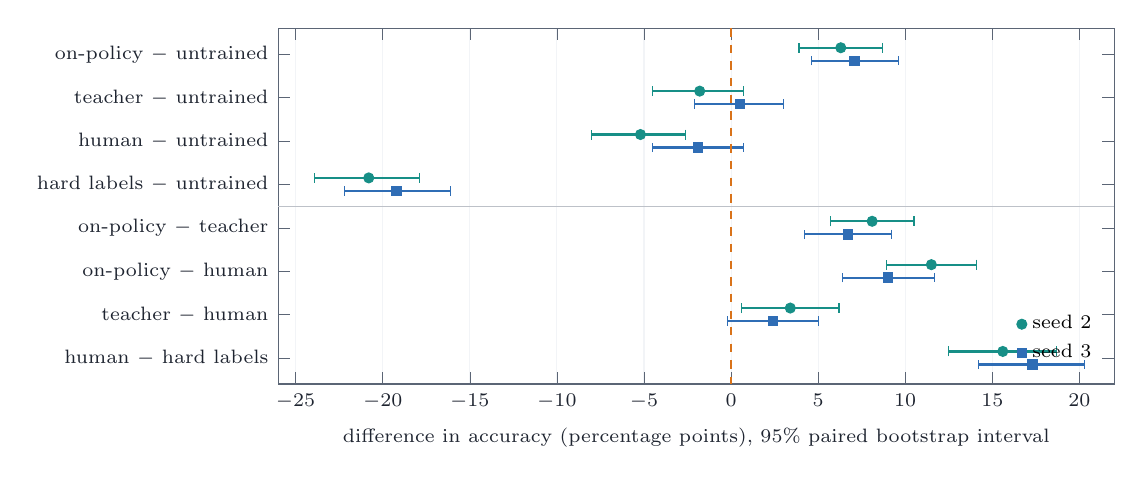
\begin{tikzpicture}
    \begin{axis}[kdaxis,width=12.2cm,height=6.1cm,
        xmin=-26,xmax=22,ymin=0.4,ymax=8.6,y dir=reverse,
        ytick={1,...,8},
        yticklabels={on-policy $-$ untrained, teacher $-$ untrained, human $-$ untrained,
                     hard labels $-$ untrained, on-policy $-$ teacher, on-policy $-$ human,
                     teacher $-$ human, human $-$ hard labels},
        xlabel={difference in accuracy (percentage points), 95\% paired bootstrap interval},
        xmajorgrids,
        legend style={at={(0.99,0.03)},anchor=south east},legend cell align=left]
      \addplot[only marks,mark=*,mark size=1.8pt,color=kdteal,
          error bars/.cd,x dir=both,x explicit,error bar style={kdteal,thick}]
        coordinates {
          (6.3,0.85) +=(2.4,0) -=(2.4,0)
          (-1.8,1.85) +=(2.5,0) -=(2.7,0)
          (-5.2,2.85) +=(2.6,0) -=(2.8,0)
          (-20.8,3.85) +=(2.9,0) -=(3.1,0)
          (8.1,4.85) +=(2.4,0) -=(2.4,0)
          (11.5,5.85) +=(2.6,0) -=(2.6,0)
          (3.4,6.85) +=(2.8,0) -=(2.8,0)
          (15.6,7.85) +=(3.1,0) -=(3.1,0)};
      \addplot[only marks,mark=square*,mark size=1.7pt,color=kdblue,
          error bars/.cd,x dir=both,x explicit,error bar style={kdblue,thick}]
        coordinates {
          (7.1,1.15) +=(2.5,0) -=(2.5,0)
          (0.5,2.15) +=(2.5,0) -=(2.6,0)
          (-1.9,3.15) +=(2.6,0) -=(2.6,0)
          (-19.2,4.15) +=(3.1,0) -=(3.0,0)
          (6.7,5.15) +=(2.5,0) -=(2.5,0)
          (9.0,6.15) +=(2.7,0) -=(2.6,0)
          (2.4,7.15) +=(2.6,0) -=(2.6,0)
          (17.3,8.15) +=(3.0,0) -=(3.1,0)};
      \draw[kdorange,dashed,thick] (axis cs:0,0.4) -- (axis cs:0,8.6);
      \draw[kdgray!40] (axis cs:-26,4.5) -- (axis cs:22,4.5);
      \legend{seed 2, seed 3}
    \end{axis}
  \end{tikzpicture}

  \scriptsize Interval clear of 0 = a real difference on these questions. Not clear of 0:
  teacher vs untrained (both seeds), human vs untrained (seed 3), teacher vs human (seed 3).
\end{frame}

% ------------------------------------------------------------- E3
\begin{frame}{What each arm cost\hfill\ours\ \who{E3}}
  \begin{columns}[c]
    \begin{column}{0.56\textwidth}
      \centering
      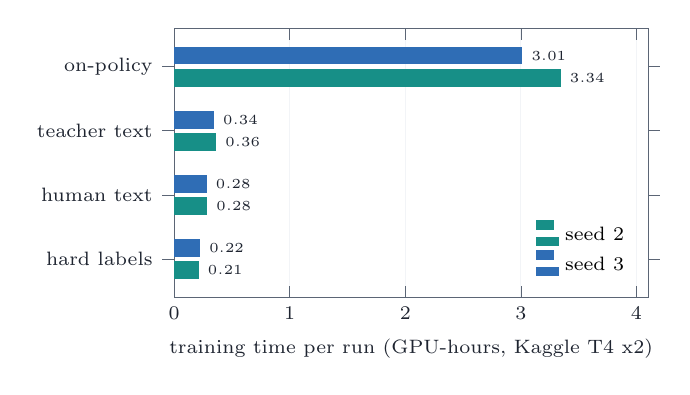
\begin{tikzpicture}
        \begin{axis}[kdaxis,width=7.6cm,height=5.0cm,
            xbar,bar width=6pt,xmin=0,xmax=4.1,
            symbolic y coords={hardlabel,human,teacher,onpolicy},ytick=data,
            yticklabels={hard labels,human text,teacher text,on-policy},
            xlabel={training time per run (GPU-hours, Kaggle T4 x2)},
            enlarge y limits=0.2,xmajorgrids,
            point meta=x,
            nodes near coords={\pgfmathprintnumber[fixed,precision=2]{\pgfplotspointmeta}},
            nodes near coords style={font=\tiny,text=kdink},
            legend style={at={(0.98,0.04)},anchor=south east},legend cell align=left]
          \addplot[fill=kdteal,draw=kdteal] coordinates
            {(0.208,hardlabel) (0.281,human) (0.358,teacher) (3.339,onpolicy)};
          \addplot[fill=kdblue,draw=kdblue] coordinates
            {(0.219,hardlabel) (0.277,human) (0.339,teacher) (3.007,onpolicy)};
          \legend{seed 2, seed 3}
        \end{axis}
      \end{tikzpicture}
    \end{column}
    \begin{column}{0.41\textwidth}
      \small
      \begin{itemize}
        \item Equal \emph{updates}, not equal \emph{compute}: on-policy
              training took about \textbf{10$\times$} longer.
        \item Equal updates are not equal tokens either: per run the
              student saw 190k answer tokens of human text, 521k of
              teacher text and about 560k of its own.
        \item Seeds 2 and 3 together: 8.0 GPU-hours of training and
              6.9 of evaluation (34 to 60 minutes per run).
      \end{itemize}
    \end{column}
  \end{columns}
\end{frame}

% ------------------------------------------------------------------
\begin{frame}{Answers got longer, and more were cut off\hfill\ours\ \who{E3}}
  \centering\footnotesize
  \renewcommand{\arraystretch}{1.2}
  \begin{tabular}{@{}l rr rr rr@{}}
    \toprule
    & \multicolumn{2}{c}{\textbf{Mean tokens}} & \multicolumn{2}{c}{\textbf{Median tokens}} & \multicolumn{2}{c}{\textbf{Cut off at 512 (\%)}} \\
    \cmidrule(lr){2-3}\cmidrule(lr){4-5}\cmidrule(l){6-7}
    \textbf{Arm} & seed 2 & seed 3 & seed 2 & seed 3 & seed 2 & seed 3 \\
    \midrule
    \arm{human}          & 259 & 290 & 239 & 270 & 5.9 & 6.8 \\
    \arm{teacher}        & 268 & 285 & 252 & 268 & 4.1 & 6.4 \\
    \arm{onpolicy}       & 282 & 304 & 260 & 282 & 8.3 & 10.1 \\
    \arm{ref\_hardlabel} & 110 & 147 & 83 & 93 & 5.0 & 12.1 \\
    \midrule
    \arm{ref\_student0}  & \multicolumn{2}{c}{232} & \multicolumn{2}{c}{217} & \multicolumn{2}{c}{1.7} \\
    \bottomrule
  \end{tabular}

  \vspace{0.25cm}
  \begin{itemize}\small
    \item All distilled students write longer answers than before training, and
          4 to 12\% of them hit the 512-token cap (1.7\% before).
    \item Hard labels taught GSM8K's short style (median under 100 tokens), yet
          5 to 12\% of answers still ran to the cap.
    \item A cut-off answer is almost always wrong, so the cap costs every arm some
          accuracy, on-policy the most.
  \end{itemize}
\end{frame}

% ------------------------------------------------------------------
\begin{frame}{Is the gain just answer length?\hfill\ours\ \who{E3}}
  \begin{columns}[c]
    \begin{column}{0.58\textwidth}
      \centering
      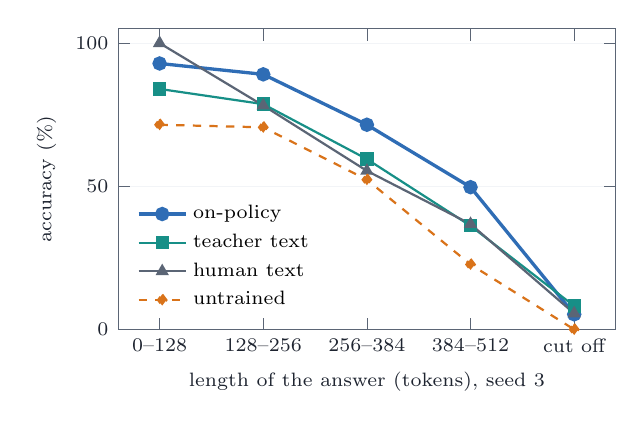
\begin{tikzpicture}
        \begin{axis}[kdaxis,width=7.9cm,height=5.4cm,
            ymin=0,ymax=105,
            symbolic x coords={a,b,c,d,e},xtick=data,
            xticklabels={0--128,128--256,256--384,384--512,cut off},
            xlabel={length of the answer (tokens), seed 3},
            ylabel={accuracy (\%)},
            ymajorgrids,legend style={at={(0.02,0.03)},anchor=south west},legend cell align=left]
          \addplot[kdblue,very thick,mark=*] coordinates
            {(a,92.9) (b,89.1) (c,71.5) (d,49.7) (e,5.3)};
          \addplot[kdteal,thick,mark=square*] coordinates
            {(a,84.0) (b,78.7) (c,59.5) (d,36.2) (e,8.2)};
          \addplot[kdgray,thick,mark=triangle*] coordinates
            {(a,100.0) (b,78.2) (c,55.4) (d,36.8) (e,5.6)};
          \addplot[kdorange,thick,dashed,mark=diamond*] coordinates
            {(a,71.5) (b,70.6) (c,52.3) (d,22.7) (e,0.0)};
          \legend{on-policy, teacher text, human text, untrained}
        \end{axis}
      \end{tikzpicture}
    \end{column}
    \begin{column}{0.39\textwidth}
      \small
      \begin{itemize}
        \item Longer answers are harder for every model.
        \item But in the two biggest bands, 128 to 384 tokens (about 80\% of
              questions), on-policy leads in \textbf{both} seeds.
        \item So the gain is not only ``shorter answers''.
      \end{itemize}
      {\tiny\color{kdgray} Band sizes differ per run; the shortest band has only
      14 to 130 answers. From \texttt{accuracy\_by\_length} in \texttt{kd/stats.py}.}
    \end{column}
  \end{columns}
\end{frame}

% ------------------------------------------------------------------
\begin{frame}{Size, speed and fidelity\hfill\ours\ \who{E3}}
  \begin{columns}[T]
    \begin{column}{0.48\textwidth}
      \begin{block}{Accuracy vs size and speed (B3 theme)}
        \footnotesize
        \renewcommand{\arraystretch}{1.2}
        \begin{tabular}{@{}lrr@{}}
          & Qwen3-4B & Qwen3-0.6B \\
          \midrule
          Parameters & 4.0 B & 0.6 B \\
          GPU memory to run (fp16) & 7.7 GB & 1.3 GB \\
          Time for 300 questions & 730 s & 321 s \\
          Accuracy, 300 questions & 83.0\% & 56.7\% \\
          Best distilled, 1,319 qs & & 69.1\% \\
        \end{tabular}

        \vspace{0.1cm}
        \scriptsize About 6.7$\times$ fewer parameters and 2.3$\times$ faster
        (headroom test, one T4, 384 tokens).
      \end{block}
    \end{column}
    \begin{column}{0.48\textwidth}
      \begin{todobox}{Teacher on the full test set (E2), then agreement (E1)}
        Run \arm{ref\_teacher} with \repofile{scripts/30\_evaluate.py}. It gives:
        \begin{itemize}
          \item teacher accuracy on all 1,319 questions (replaces the 300-question numbers);
          \item \textbf{agreement}: how often each student's final answer equals the
                teacher's, overall and on questions the teacher gets wrong
                (\texttt{agreement()} in \repofile{kd/stats.py});
          \item the teacher's evaluation time at 512 tokens, for the speed row.
        \end{itemize}
      \end{todobox}
    \end{column}
  \end{columns}
\end{frame}

% =====================================================================
% 08-interpretation.tex -- Interpretation and limitations.
% E1 2 min (what the results show), E3 3 min (limitations and
% alternative explanations). DRAFT: based on seeds 2 and 3 only; update
% after seed 1 and the interpretation meeting.
% =====================================================================
\renewcommand{\sectioninfo}{Presenters: E1 (2 min), E3 (3 min)}
\section{Interpretation and limitations}

% ------------------------------------------------------------- E1
\begin{frame}{What the results show (draft, two seeds)\hfill\ours\ \who{E1}}
  \small
  \begin{enumerate}
    \item<1-> \textbf{The source of the text matters.} With the same target and the same
          500 updates, the student's own text gave \textbf{+6.3 and +7.1 points} over the
          untrained student and +6.7 to +11.5 over the other two sources; every one of these
          intervals excludes 0.
    \item<2-> \textbf{Off-policy text did not help here.} Teacher text: $-1.8$ and $+0.5$
          (not significant); human text: $-5.2$ (significant) and $-1.9$ (not).
          The already tuned student had little to gain from imitating fixed text.
    \item<3-> \textbf{Soft targets matter.} On the same human text, matching the teacher's
          distribution beat hard labels by \textbf{+15.6 and +17.3 points}: the classic
          B3 result, reproduced at this scale.
  \end{enumerate}
  \vspace{0.15cm}
  \begin{uncoverenv}<4->
  \begin{keybox}
    \footnotesize This pattern \emph{fits} the exposure-bias explanation: only the arm that
    learns on its own prefixes improves. It does not \emph{prove} it; the next slide
    lists what else could produce the same numbers.
  \end{keybox}
  \end{uncoverenv}
  \begin{uncoverenv}<4->
  \begin{todobox}{Final wording after seed 1 and the interpretation meeting (E1)}
    Check that seed 1 shows the same pattern; then fix the wording here and in the note.
  \end{todobox}
  \end{uncoverenv}
\end{frame}

% ------------------------------------------------------------- E3
\begin{frame}{Limitations and alternative explanations\hfill\who{E3}}
  \begin{columns}[T]
    \begin{column}{0.49\textwidth}
      \begin{block}{Could something else explain the gain?}
        \footnotesize
        \begin{itemize}
          \item \textbf{Compute}: on-policy used about 10$\times$ the training
                time. A compute-matched comparison would be fairer to the
                other arms.
          \item \textbf{Tuning}: the learning rate was picked on the on-policy
                arm and on the test set, which may favour it slightly.
          \item \textbf{Tokens}: equal updates gave the arms different
                numbers of answer tokens (190k to 566k).
          \item \textbf{Length}: on-policy answers are longer, but it still
                leads within each of the two main length bands.
        \end{itemize}
      \end{block}
    \end{column}
    \begin{column}{0.47\textwidth}
      \begin{block}{What our design cannot tell us}
        \footnotesize
        \begin{itemize}
          \item One dataset (GSM8K), one model pair from one family.
          \item Three seeds at most (two so far); 500 updates only.
          \item Distillation temperature fixed at 1; forward KL only.
          \item Qwen models may have seen GSM8K in pre-training
                \src{Wu et al., 2025}; it affects all arms alike.
          \item Teacher answers were greedy and not filtered for
                correctness (92.1\% correct).
        \end{itemize}
      \end{block}
    \end{column}
  \end{columns}
  \vspace{0.1cm}
  \begin{todobox}{E3: choose the three limitations to say out loud (3 minutes)}
    Fill \repofile{notes/theory/e3-compression-and-contamination.md}; keep the rest for questions.
  \end{todobox}
\end{frame}

% =====================================================================
% 09-conclusion.tex -- Conclusion and reproducibility.  E3, 3 min
% Sources: repository layout on main, scripts/20_train.py,
%          notebooks/kaggle_run.ipynb, results/run_log.csv
% =====================================================================
\renewcommand{\sectioninfo}{Presenter: E3 \quad $\cdot$ \quad 3 minutes}
\section{Conclusion and reproducibility}

% ------------------------------------------------------------------
\begin{frame}[fragile]{Reproduce everything from the repository\hfill\who{E3}}
  \begin{columns}[T]
    \begin{column}{0.47\textwidth}
\begin{lstlisting}[style=kdplain]
configs/    default.yaml, smoke.yaml
data/       teacher_sequences.jsonl
src/kd/     data, answer_extraction, losses,
            train, evaluate, stats
scripts/    10_cache_teacher_sequences.py
            20_train.py   30_evaluate.py
            40_make_figures.py
notebooks/  kaggle_run.ipynb, archive/
tests/      one pytest file per module
results/    run_log.csv, runs/<run_id>/
report/     note.qmd, references.bib, slides/
\end{lstlisting}
    \end{column}
    \begin{column}{0.5\textwidth}
\begin{lstlisting}[style=kdplain,language=bash,basicstyle=\ttfamily\tiny]
pip install -r requirements.txt && pip install -e .
CFG=configs/default.yaml
python scripts/10_cache_teacher_sequences.py --config $CFG
python scripts/20_train.py --config $CFG --arm onpolicy --seed 1
python scripts/30_evaluate.py --config $CFG --run onpolicy_s1
python -m kd.stats --out results/tables/results_table.csv
\end{lstlisting}
      \footnotesize
      \begin{itemize}
        \item \repofile{configs/smoke.yaml}: the same pipeline on 16 questions,
              about 15 minutes.
        \item Teacher answers and every run's predictions are committed, so the
              statistics rerun without a GPU.
      \end{itemize}
    \end{column}
  \end{columns}
  \begin{todobox}{README and figure script (E3)}
    \repofile{README.md} is still the 2-line stub and
    \repofile{scripts/40\_make\_figures.py} is empty on \repofile{main}; both are
    required by the brief.
  \end{todobox}
\end{frame}

% ------------------------------------------------------------------
\begin{frame}[fragile]{Every number traces back to code and settings\hfill\ours\ \who{E3}}
  \begin{columns}[T]
    \begin{column}{0.52\textwidth}
\begin{lstlisting}
# scripts/20_train.py records every run (shortened)
info = {
    "run_id": run_id, "arm": args.arm,
    "seed": args.seed, "started_utc": utc_now(),
    "git_commit": git_commit(),     # "+dirty" if edited
    "config_hash": file_hash(cfg),  # sha256 of the file
}
update_run_log(run_id, status="running", **info)
summary = run_training(cfg, arm, seed, out_dir)
# finally: status, end time, GPU-hours -> run_info.json
\end{lstlisting}
    \end{column}
    \begin{column}{0.45\textwidth}
      \footnotesize
      \begin{itemize}
        \item One row per run in \repofile{results/run\_log.csv}, one folder per run
              in \repofile{results/runs/}.
        \item All 8 main runs so far: commit \texttt{f2accc6}, config hash
              \texttt{85bee6cac023}: identical code and settings.
        \item On Kaggle, \repofile{notebooks/kaggle\_run.ipynb} only clones that
              commit and calls the scripts: no logic hidden in a notebook.
        \item Checkpoints stay on Kaggle; only small result files enter git.
      \end{itemize}
    \end{column}
  \end{columns}
\end{frame}

% ------------------------------------------------------------------
\begin{frame}{Conclusion\hfill\who{E3}}
  \begin{columns}[T]
    \begin{column}{0.55\textwidth}
      \begin{keybox}
        \small At equal updates and with the same target, \textbf{the student's own text}
        was the only source that made Qwen3-0.6B better at GSM8K: about
        \textbf{+7 points} over the untrained model in both seeds so far, while human
        and teacher text gave no gain. Matching the teacher's \textbf{probabilities}
        rather than hard labels was worth about \textbf{+16 points}.
      \end{keybox}
      \vspace{0.1cm}
      {\scriptsize\color{kdgray} Draft based on seeds 2 and 3; confirm with seed 1.}
    \end{column}
    \begin{column}{0.42\textwidth}
      \begin{block}{Next steps we did not run}
        \footnotesize
        \begin{itemize}
          \item A compute-matched comparison
          \item Reverse KL and mixed on/off-policy batches
          \item Other distillation temperatures
          \item A same-size teacher (Born-Again setting)
          \item A second dataset or model family
        \end{itemize}
      \end{block}
    \end{column}
  \end{columns}
  \vspace{0.15cm}
  \begin{todobox}{Final take-home message (E3 with the team)}
    Agree on one sentence the audience should remember, after seed 1 and the interpretation meeting.
  \end{todobox}
\end{frame}

% ------------------------------------------------------------------
\begin{frame}[plain,noframenumbering]
  \begin{tikzpicture}[remember picture,overlay]
    \fill[kdpaler] (current page.north west) rectangle (current page.south east);
    \fill[kdblue] (current page.north west) rectangle ([xshift=0.22cm]current page.south west);
  \end{tikzpicture}%
  \centering
  \vspace{1.2cm}
  {\color{kdnavy}\Huge\bfseries Questions?\par}
  \vspace{0.5cm}
  {\color{kdblue}\large Whose text should a small model practise on?\par}
  \vspace{0.8cm}
  {\small\color{kdgray} Code, results and this deck:
  \texttt{github.com/redkitex/Knowledge-Distillation-and-Model-Compression}\par}
\end{frame}


\appendix
% =====================================================================
% 10-backup.tex -- Backup slides (not counted in the 60 minutes) and
% references. Owner: T3; references: E2.
% =====================================================================
\renewcommand{\sectioninfo}{Backup slides and references}
\section{Backup}

% ------------------------------------------------------------------
\begin{frame}{Backup: all pilot runs (seed 1, 100 steps)\hfill\ours}
  \centering\footnotesize
  \renewcommand{\arraystretch}{1.2}
  \begin{tabular}{@{}l l r r r@{}}
    \toprule
    \textbf{Run} & \textbf{Arm} & \textbf{lr} & \textbf{sampling $T$} & \textbf{Accuracy (\%)} \\
    \midrule
    \arm{pilot\_human\_s1}         & human         & $1\cdot10^{-5}$ & --  & 51.0 \\
    \arm{pilot\_teacher\_s1}       & teacher       & $1\cdot10^{-5}$ & --  & 54.4 \\
    \arm{pilot\_ref\_hardlabel\_s1} & ref\_hardlabel & $1\cdot10^{-5}$ & --  & 29.6 \\
    \midrule
    \arm{pilot\_onpolicy\_lr1e-05\_t0.7\_s1} & onpolicy & $1\cdot10^{-5}$ & 0.7 & 60.6 \\
    \arm{pilot\_onpolicy\_lr2e-05\_t0.7\_s1} & onpolicy & $2\cdot10^{-5}$ & 0.7 & 50.2 \\
    \arm{pilot\_onpolicy\_lr5e-06\_t0.5\_s1} & onpolicy & $5\cdot10^{-6}$ & 0.5 & 64.5 \\
    \arm{pilot\_onpolicy\_lr5e-06\_t0.7\_s1} & onpolicy & $5\cdot10^{-6}$ & 0.7 & \textbf{65.6} \\
    \arm{pilot\_onpolicy\_lr5e-06\_t1\_s1}   & onpolicy & $5\cdot10^{-6}$ & 1.0 & 63.5 \\
    \midrule
    \arm{ref\_student0} & untrained & -- & -- & 62.0 \\
    \bottomrule
  \end{tabular}

  \vspace{0.2cm}
  \raggedright\scriptsize
  At $1\cdot10^{-5}$ every off-policy pilot fell below the untrained student, which led to the
  sweep and to $5\cdot10^{-6}$ for all main runs. Pilots and main runs used different learning
  rates, so their numbers are not compared with each other. All 8 pilots saw identical
  questions in identical order.
\end{frame}

% ------------------------------------------------------------------
\begin{frame}[fragile]{Backup: running one arm on Kaggle\hfill\who{T3}}
  \begin{columns}[T]
    \begin{column}{0.58\textwidth}
\begin{lstlisting}[basicstyle=\ttfamily\tiny]
# notebooks/kaggle_run.ipynb, settings cell
REPO = "https://github.com/redkitex/Knowledge-Distillation-and-Model-Compression.git"
REF = "f2accc6"                # same commit for every seed
CONFIG = "configs/default.yaml"
MODE = "train+eval"            # or "eval" for references
ARM = "onpolicy"               # human | teacher | onpolicy | ref_hardlabel
SEED = 3
RUN_ID = None                  # -> "onpolicy_s3"
ACCOUNT = "T3"                 # whose Kaggle account
MAX_STEPS = None               # None = the full 500 steps
\end{lstlisting}
    \end{column}
    \begin{column}{0.39\textwidth}
      \footnotesize
      \begin{enumerate}
        \item Session options: GPU T4 x2, internet on.
        \item Edit the settings cell only.
        \item Save Version, Save \& Run All: clone, install, train, evaluate.
        \item Download \texttt{<run\_id>.zip} from the output; copy the row
              from \texttt{run\_info.json} into \repofile{results/run\_log.csv}.
      \end{enumerate}
      \vspace{0.1cm}
      {\scriptsize\color{kdgray} One free account runs one GPU session at a time:
      start the 3-hour on-policy run first.}
    \end{column}
  \end{columns}
\end{frame}

% ------------------------------------------------------------------
\begin{frame}{Backup: how the project ran\hfill\who{T3}}
  \centering
  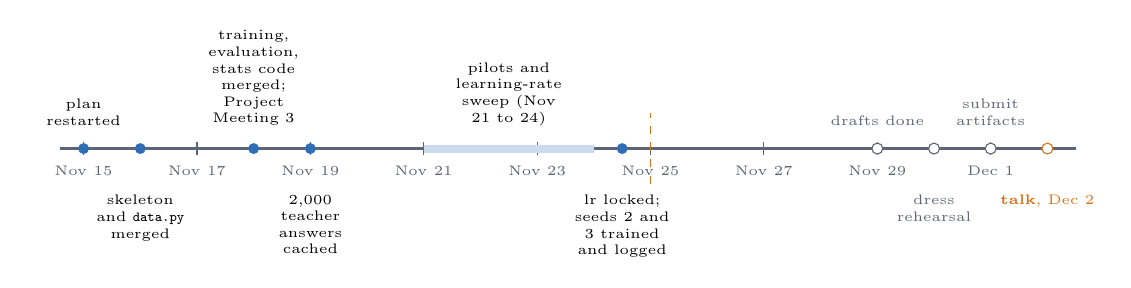
\begin{tikzpicture}[font=\tiny,
      ev/.style={text width=1.35cm,align=center,inner sep=1pt},
      done/.style={circle,fill=kdblue,inner sep=1.4pt},
      plan/.style={circle,draw=kdgray,fill=white,inner sep=1.4pt}]
    \def\ux{0.72}
    \draw[kdgray,thick] (-0.3,0) -- (12.6,0);
    % day ticks every two days, labelled
    \foreach \dd/\lab in {0/15,2/17,4/19,6/21,8/23,10/25,12/27,14/29}
      {\draw[kdgray] (\dd*\ux,-0.08) -- (\dd*\ux,0.08);
       \node[text=kdgray,below=0.1cm] at (\dd*\ux,0) {Nov \lab};}
    \draw[kdgray] (16*\ux,-0.08) -- (16*\ux,0.08);
    \node[text=kdgray,below=0.1cm] at (16*\ux,0) {Dec 1};
    % pilots range
    \fill[kdblue!25] (6*\ux,-0.05) rectangle (9*\ux,0.05);
    % events above
    \node[done] at (0,0) {};             \node[ev,above=0.25cm] at (0,0) {plan restarted};
    \node[done] at (3*\ux,0) {};         \node[ev,above=0.25cm] at (3*\ux,0) {training, evaluation, stats code merged; Project Meeting 3};
    \node[ev,above=0.25cm] at (7.5*\ux,0) {pilots and learning-rate sweep (Nov 21 to 24)};
    \node[plan] at (14*\ux,0) {};        \node[ev,above=0.25cm,text=kdgray] at (14*\ux,0) {drafts done};
    \node[plan] at (16*\ux,0) {};        \node[ev,above=0.25cm,text=kdgray] at (16*\ux,0) {submit artifacts};
    % events below
    \node[done] at (1*\ux,0) {};         \node[ev,below=0.55cm] at (1*\ux,0) {skeleton and \texttt{data.py} merged};
    \node[done] at (4*\ux,0) {};         \node[ev,below=0.55cm] at (4*\ux,0) {2,000 teacher answers cached};
    \node[done] at (9.5*\ux,0) {};       \node[ev,below=0.55cm] at (9.5*\ux,0) {lr locked; seeds 2 and 3 trained and logged};
    \node[plan] at (15*\ux,0) {};        \node[ev,below=0.55cm,text=kdgray] at (15*\ux,0) {dress rehearsal};
    \node[plan,draw=kdorange] at (17*\ux,0) {}; \node[ev,below=0.55cm,text=kdorange] at (17*\ux,0) {\textbf{talk}, Dec 2};
    % today marker
    \draw[kdorange,dashed] (10*\ux,-0.45) -- (10*\ux,0.45);
  \end{tikzpicture}

  \vspace{0.35cm}
  \scriptsize
  \begin{tabular}{@{}llll@{}}
    \toprule
    & \textbf{1} & \textbf{2} & \textbf{3} \\
    \midrule
    \textbf{Training team} (builds, runs) & T1 training loop & T2 data, teacher answers & T3 runs, configs, slides \\
    \textbf{Evaluation team} (measures, explains) & E1 statistics, note & E2 evaluation, literature & E3 figures, repository \\
    \bottomrule
  \end{tabular}
  \vspace{0.1cm}

  {\scriptsize\color{kdgray} Filled dots: done (from the commit history); open dots: planned; dashed line: Nov 25.}
\end{frame}

% ------------------------------------------------------------------
\begin{frame}{References\hfill\who{E2}}
  \begin{columns}[T]
    \begin{column}{0.49\textwidth}
      \tiny
      \begin{itemize}\setlength{\itemsep}{1pt}
        \item Agarwal et al. (2024). On-Policy Distillation of Language Models: Learning from Self-Generated Mistakes. ICLR.
        \item Bengio, Vinyals, Jaitly, Shazeer (2015). Scheduled Sampling for Sequence Prediction with Recurrent Neural Networks. NeurIPS.
        \item Brown, Cai, DasGupta (2001). Interval Estimation for a Binomial Proportion. Statistical Science.
        \item Cobbe et al. (2021). Training Verifiers to Solve Math Word Problems. arXiv.
        \item DeepSeek-AI (2025). DeepSeek-R1: Incentivizing Reasoning Capability in LLMs via Reinforcement Learning. arXiv.
        \item Efron, Tibshirani (1993). An Introduction to the Bootstrap. Chapman \& Hall.
        \item Furlanello et al. (2018). Born Again Neural Networks. ICML.
        \item Gu, Dong, Wei, Huang (2024). MiniLLM: Knowledge Distillation of Large Language Models. ICLR.
        \item Hinton, Vinyals, Dean (2015). Distilling the Knowledge in a Neural Network. arXiv.
        \item Kim, Rush (2016). Sequence-Level Knowledge Distillation. EMNLP.
      \end{itemize}
    \end{column}
    \begin{column}{0.49\textwidth}
      \tiny
      \begin{itemize}\setlength{\itemsep}{1pt}
        \item Li et al. (2026). Rethinking On-Policy Distillation of Large Language Models: Phenomenology, Mechanism, and Recipe. arXiv.
        \item Lu, Thinking Machines Lab (2025). On-Policy Distillation. Blog post.
        \item Miller (2024). Adding Error Bars to Evals: A Statistical Approach to Language Model Evaluations. arXiv.
        \item Qwen Team (2025). Qwen3 Technical Report. arXiv.
        \item Ross, Gordon, Bagnell (2011). A Reduction of Imitation Learning and Structured Prediction to No-Regret Online Learning. AISTATS.
        \item Song, Zheng (2026). A Survey of On-Policy Distillation for Large Language Models. arXiv.
        \item Stanton et al. (2021). Does Knowledge Distillation Really Work? NeurIPS.
        \item Wilson (1927). Probable Inference, the Law of Succession, and Statistical Inference. JASA.
        \item Wu et al. (2025). Reasoning or Memorization? Unreliable Results of Reinforcement Learning Due to Data Contamination. arXiv.
      \end{itemize}
    \end{column}
  \end{columns}
  \vspace{0.1cm}
  \begin{todobox}{Verify every reference (E2)}
    The course requires checking authors, year and venue against each paper. Ross 2011, Li 2026 and
    Song and Zheng 2026 are not yet in \repofile{report/references.bib}.
  \end{todobox}
\end{frame}


\end{document}
